%%%%%%%%%%%%%%%%%%%%%%%%%%%%%%%%%%%%%%%%%
% Beamer Presentation
% LaTeX Template
% Version 1.0 (10/11/12)
%
% This template has been downloaded from:
% http://www.LaTeXTemplates.com
%
% License:
% CC BY-NC-SA 3.0 (http://creativecommons.org/licenses/by-nc-sa/3.0/)
%
%%%%%%%%%%%%%%%%%%%%%%%%%%%%%%%%%%%%%%%%%

%----------------------------------------------------------------------------------------
%	PACKAGES AND THEMES
%----------------------------------------------------------------------------------------

\documentclass{beamer}
\mode<presentation> {
\usetheme{Madrid}
\usefonttheme{serif} 
\setbeamertemplate{navigation symbols}{} % To remove the navigation symbols from the bottom of all}
}
\usepackage{graphicx} % Allows including images
\usepackage{booktabs} % Allows the use of \toprule, \midrule and \bottomrule in tables
\usepackage[T1]{fontenc}
\usepackage[utf8]{inputenc}
\usepackage{amsmath}
\usepackage{color}
\usepackage[czech]{babel}
\usepackage{lmodern}  
\usepackage{rotating}
\usepackage{scrextend}
\usepackage{pifont}
\usepackage{hyperref}
\usepackage{pifont}
\usepackage{bm}

%----------------------------------------------------------------------------------------
%	TITLE PAGE
%----------------------------------------------------------------------------------------

\title[Block 2]{Praktikum z ekonometrie} % The short title appears at the bottom of every slide, the full title is only on the title page

\author{VŠE Praha} % Your name
\institute[4EK417] % Your institution as it will appear on the bottom of every slide, may be shorthand to save space
{
% Your institution for the title page
\medskip
\textit{Tomáš Formánek} % Your email address
}
\date{} % Date, can be changed to a custom date

\begin{document}

\begin{frame}
\titlepage % Print the title page as the first slide
\end{frame}

\begin{frame}
\frametitle{Block 2 -- Model selection -- Outline} % Table of contents slide, comment this block out to remove it
\tableofcontents % Throughout your presentation, if you choose to use \section{} and \subsection{} commands, these will automatically be printed on this slide as an overview of your presentation
\end{frame}

%---------------------------------------------
\section{Model selection}
\begin{frame}{Theoretical basis for model selection algorithms}

\end{frame}
%---------------------------------------------
\subsection{Theoretical approach: specific-to-general, general-to-specific}
\begin{frame}{Alternative approaches to econometric modeling}
Simple-to-general approach\\
\vspace{0.3cm}
\begin{itemize}
\item Traditional approach to econometric modeling
\vspace{0.3cm}
\item Starts with formulation of the simplest model consistent with the relevant economic theory.
\vspace{0.3cm}
\item If this initial model proves unsatisfactory, it is improved in some way – adding or changing variables, using different estimators etc.
\end{itemize}
\end{frame}
%---------------------------------------------
\begin{frame}{Alternative approaches to econometric modeling}
 Criticism  of the simple-to-general approach\\
\begin{itemize}
\vspace{0.3cm}
\item Revisions to the simple model are carried out arbitrarily and simply reflect investigator's prior beliefs: danger of always finding what you want to find.
\vspace{0.3cm}
\item It is open to accusation of data mining: researchers usually presents just the final model (true significance level is problematic).
\end{itemize}
\end{frame}
%---------------------------------------------
\begin{frame}{Alternative approaches to econometric modeling}
General-to-specific approach\\
\medskip
\begin{itemize}
\item Professor Hendry, London School of Economics \\started this approach in the 80ies.
\medskip
\item It starts with formulation of a very general and maybe quite complicated model.
\medskip
\item Starting model contains a series of simpler models, nested within it as special cases. 
\medskip
\item These simpler models should represent all the alternative economic hypotheses that require consideration.
\end{itemize}
\end{frame}
%---------------------------------------------
\begin{frame}{Alternative approaches to econometric modeling}
General-to-specific approach\\
\vspace{0.3cm}
\begin{itemize}
\item General model must be able to explain existing data and be able to satisfy various tests of misspecification.
\vspace{0.3cm}
\item What follows is simplification search (testing-down procedure). Through parameter restrictions, we test nested models against the containing model. If the nested model does not pass the tests, we can reject the whole branch of sub-nested models.
\vspace{0.3cm}
\item If we find more non-nested models satisfying tests, we can compare those (using information criteria, etc.).
\end{itemize}
\end{frame}
%---------------------------------------------
\begin{frame}{Alternative approaches to econometric modeling}
Advantages of the general-to-specific approach\\
\vspace{0.3cm}
\begin{itemize}
\item ``Data mining''  present in this approach is transparent (for all to see) and it is carried out in a systematic manner that avoids worst data mining problems. 
\vspace{0.3cm}
\item Researcher usually reports both the initial general model and all steps involved so it is possible to get some idea about the true significance levels.
\vspace{0.3cm}
\item Supporters of this approach stress the importance of both testing final models against new data and the ability of the model to provide adequate out-of-sample forecasts.
\end{itemize}
\end{frame}
%---------------------------------------------
\begin{frame}{Model selection basics - repetition from previous courses}
\end{frame}
%---------------------------------------------
\begin{frame}{Variance vs. Bias trade-off - repetition}
Population equation example: $~y = \textnormal{sin}(x)+u$
\vspace{-1cm}
\begin{figure}
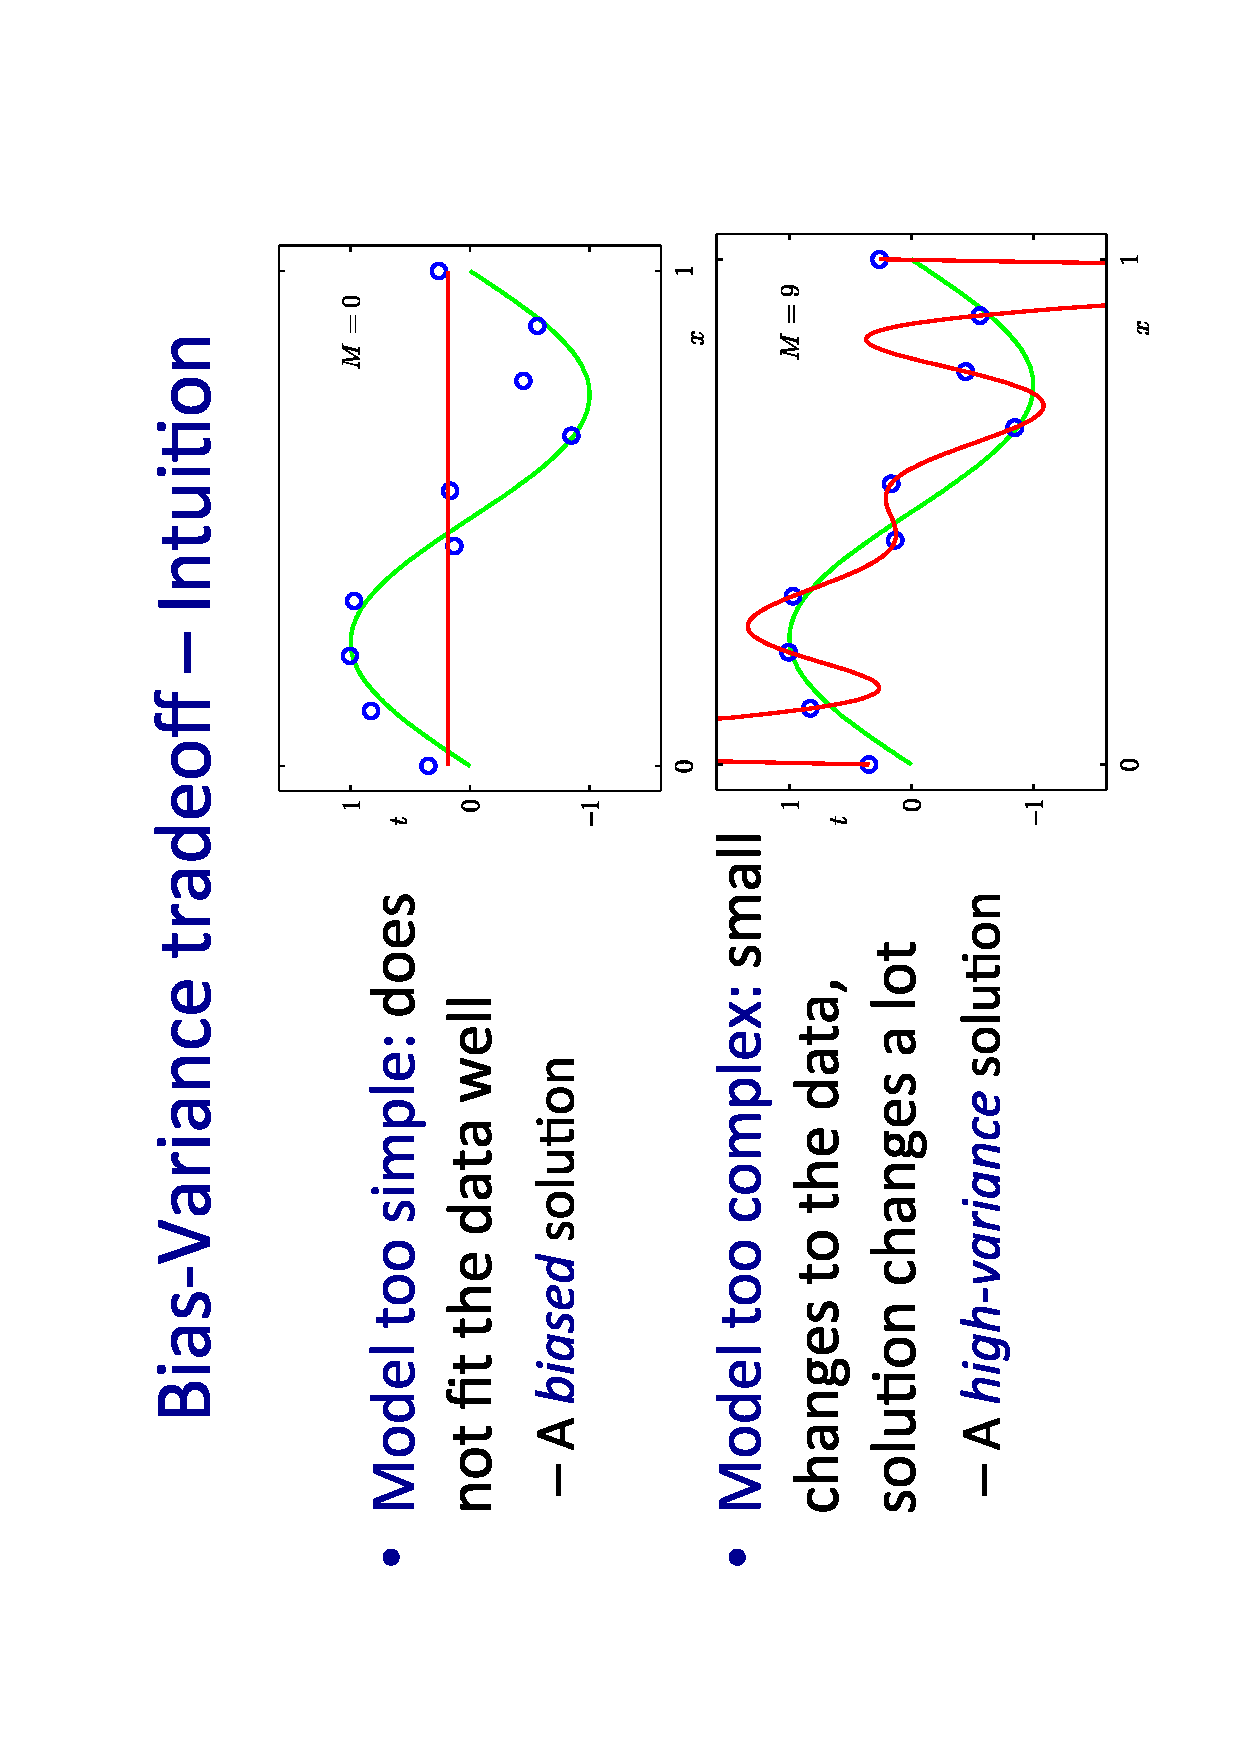
\includegraphics[angle=270,scale=0.35]{IMG/VarBias.pdf}
\end{figure}
\end{frame}
%---------------------------------------------
\begin{frame}{Train sample \& Test sample - repetition}

Suppose we fit a model $\hat{f}(\bm{x})$ to some training data $\textnormal{Tr}=\left\lbrace y_i, \bm{x}_i \right\rbrace _1 ^n$ and we wish to see how well it performs.

\begin{itemize}
\item We could compute $\textit{MSE}$ over $\textnormal{Tr}$:
$$ \textit{MSE}_{\textnormal{Tr}} = \frac{1}{n}
   \sum_{i \in \textnormal{Tr}}
   \left[y_i - \hat{f}(\bm{x}_i) \right]^2 $$
\end{itemize}

When searching for the ``best'' model by minimizing $ \textit{MSE}$, the above statistic would lead to over-fit models.
\vspace{0.3cm}
\begin{itemize}
\item Instead, we should (if possible) compute the $ \textit{MSE}$ using fresh test
data $\textnormal{Te}=\left\lbrace y_i, \bm{x}_i \right\rbrace _1 ^m$:
$$ \textit{MSE}_{\textnormal{Te}} = \frac{1}{m}
    \sum_{i \in \textnormal{Te}}
   \left[y_i - \hat{f}(\bm{x}_i) \right]^2 $$
\end{itemize}
\end{frame}
%---------------------------------------------
\begin{frame}{Variance vs. Bias trade-off - repetition}
\vspace{-0.5cm}
$$\textnormal{E}(\textit{MSE}_0)
   = \textit{var}(\hat{f}(\bm{x}_0))
   + [\textit{Bias\,}(\hat{f}(\bm{x}_0))]^2
   + \textnormal{var}(\varepsilon_0)$$\\
\begin{figure}
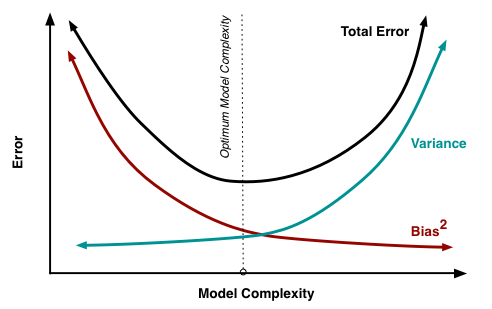
\includegraphics[angle=0,scale=0.30]{IMG/biasvariance.png}
\end{figure}
\small{This is an illustration, $\textnormal{var}(\varepsilon_0)$ not shown explicitly. \\(lies at the /asymptotic/ minima of Variance and $\textnormal{Bias}^2$)}\\
\small{
\begin{itemize}
    \item Variance refers to the amount by which $\hat{f}(\bm{x}_0)$ would change if we estimate it using different training data sets.   
    \item Bias is introduced by approximating real-life DGP by simple model.
    \item Derivation of the formula is complex, see eg. \textcolor{blue}{\underline{\href{https://stats.stackexchange.com/questions/204115/understanding-bias-variance-tradeoff-derivation}{information here}}}
\end{itemize}}
\end{frame}
%------------------------------------------------
\begin{frame}{$k$-Fold Cross Validation - repetition}
\begin{itemize}
\item Training error ($\textit{MSE}_{\textnormal{Tr}}$) can be calculated easily. 
\item However, $\textit{MSE}_{\textnormal{Tr}}$ is not a good approximation for the $\textit{MSE}_{\textnormal{Te}}$ (out-of sample predictive properties of the model).
\item Usually, $\textit{MSE}_{\textnormal{Tr}}$ dramatically underestimates $\textit{MSE}_{\textnormal{Te}}$.
\end{itemize}
\bigskip
Cross-validation is based on re-sampling (similar to bootstrap).\\
\medskip
Repeatedly fit a model of interest to samples formed from the training set \& make ``test sample'' predictions, in order to obtain additional information about predictive properties of the model.\\
\end{frame}
%---------------------------------------------
\begin{frame}{$k$-Fold Cross Validation - repetition}
\begin{itemize}
  \item In $k$-Fold Cross-Validation ($k$FCV), the original sample is randomly partitioned into $k$ roughly equal subsamples (divisibility). 
  \item Of the $k$ subsamples, a single subsample is retained as the test sample, and the remaining $(k-1)$ subsamples are used as training data. 
  \item The cross-validation process is then repeated $k$ times (the $k$ folds), with each of the $k$ subsamples used exactly once as the test sample. 
  \item The $k$ results from the folds can then be averaged to produce a single estimation -- the cross-validated error. 
  \item $k = 5$ or $k=10$ is commonly used.
  \item Sometimes, $k$FCV process is repeated ($R$-times -- say, 100) to get distribution of the cross-validated error term.
\end{itemize}  
\end{frame}
%------------------------------------------------
\begin{frame}{$k$-Fold Cross Validation - repetition}
\begin{center}
$k$FCV example for CS data \& $k=5$: \\
(random sampling, no replacement)
\begin{figure}
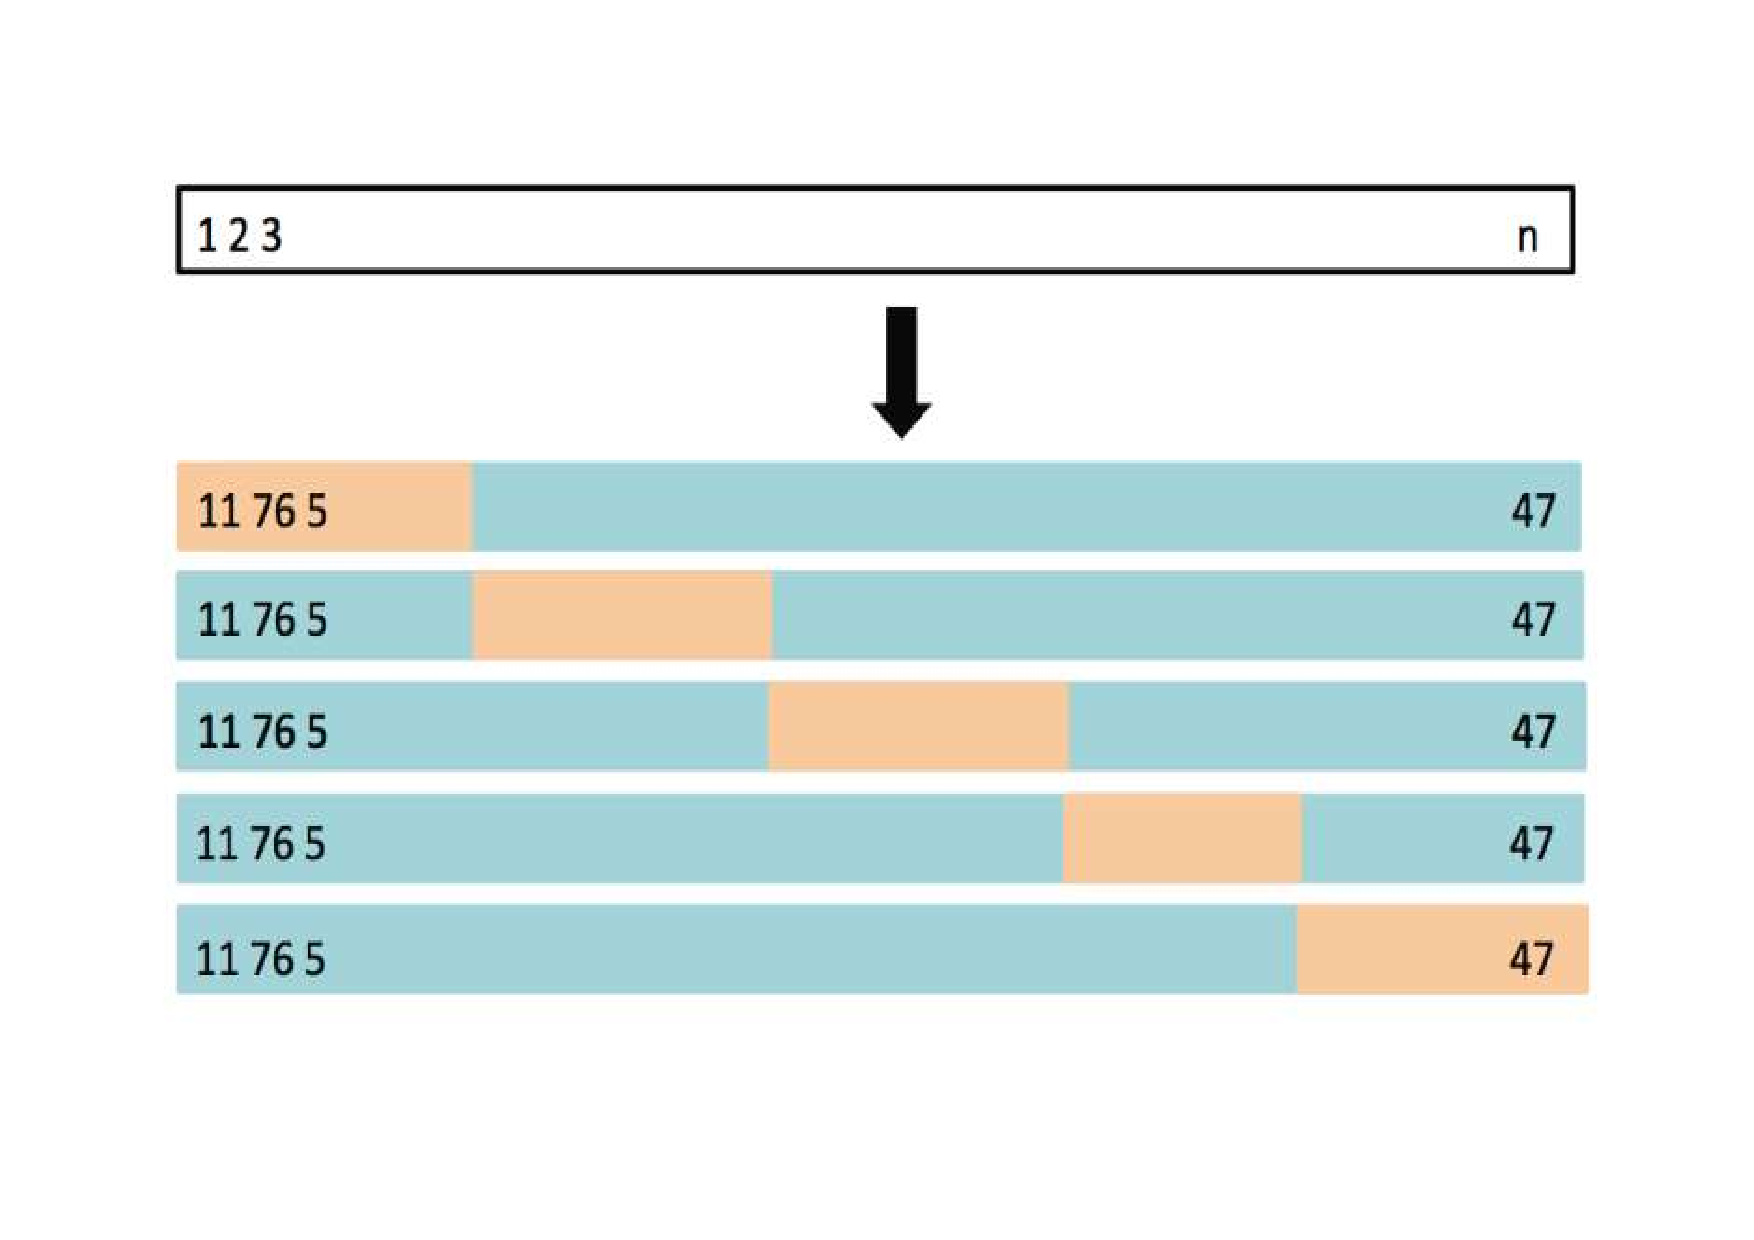
\includegraphics[width=0.7\linewidth]{IMG/kFCV2.pdf}
\end{figure}
\vspace{-1cm}
In TS, a similar ``Walk forward'' test procedure may be applied.
\end{center}
\end{frame}
%------------------------------------------------
\begin{frame}{$k$-Fold Cross Validation - repetition}
$ \textit{CV}_{(k)}= \frac{1}{k}\displaystyle\sum_{s=1}^{k} \textit{MSE}_s \,,$
\vspace{0.3cm}
\\where:
\begin{itemize}
\item [~~] $\textit{CV}_{(k)}$ is the $k$-fold \textit{CV} estimate,
\item [~~] $k$ is the number of folds used (e.g. 5 or 10),
\item [~~] $\textit{MSE}_s = \frac{1}{m_s} \sum_{i \in C_s}^{}(y_i - \widehat{y}_i)^2 $ 
\item [~~] $m_s$ and $C_s$ refer to test sample  observations for each \\of the $k$FCV steps.
\end{itemize}
\vspace{0.3cm}
As we evaluate predictions from two or more models, 
\\we look for the lowest $\textit{CV}_{(k)}$. 
\end{frame}
%---------------------------------------------
\begin{frame}{Comparison of estimation methods / models}
\textbf{Comparison of models/methods (besides \textbf{\textit{k}FCV methods} ):} 
\begin{equation} \notag
\begin{aligned}
 \textnormal{Mallow's} \hspace{0.2cm}
 \textit{C}_{p} &=\frac{1}{n}(\textit{RSS}+2d\widehat{\sigma}^2), \\
 \smallskip
 \textit{AIC} &=\frac{1}{n\widehat{\sigma}^2}(\textit{RSS}+2d\widehat{\sigma}^2), \\
 \smallskip
 \textit{BIC} &=\frac{1}{n}(\textit{RSS}+\log(n)d\widehat{\sigma}^2),
 \end{aligned}
\end{equation}

\begin{itemize}
\item where $d$ is the number of regressors and $n$ is the sample size.
\item Model selection: find a model where a statistic is minimized.
\item $\log(n)>2$ $(n\!>\!7)$ $\Rightarrow$ generally, $\textit{BIC}$ penalizes complexity more.
\item When comparing models, $\textit{AIC} \propto C_p$;~~ \\$\textit{AIC}$ and $\textit{BIC}$ may contradict 
\item If $\widehat{\sigma}^2$ is an unbiased estimate of ${\sigma}^2$, then $C_p$ is an unbiased estimate of test $\textit{MSE}$ (training error is adjusted by a factor proportional to the number of basis functions used).
\item Sometimes, models are selected using $C_p$ (\textit{AIC}) instead $k$FCV.
\end{itemize}
\end{frame}
%------------------------------------------------
\begin{frame}{Model selection algorithms}
\end{frame}
%---------------------------------------------
\begin{frame}{Model selection algorithms - Introduction}
\begin{itemize}
\item \textbf{Subset Selection:} We identify a subset of the $p$ predictors
that we believe to be related to the response. We then fit a
model using least squares on the reduced set of variables.
\medskip
\item \textbf{Shrinkage:} We fit a model involving all $p$ predictors, but
the estimated coefficients are shrunken towards zero
relative to the least squares estimates. This shrinkage (also
known as regularization) has the effect of reducing variance
and can also perform variable selection.
\medskip
\item \textbf{Dimension Reduction:} We project the $p$ predictors into a
$M$-dimensional subspace, where $M < p$. This is achieved by
computing $M$ different linear combinations, or projections,
of the variables. Then these $M$ projections are used as
predictors to fit \\a linear regression model by least squares.

\end{itemize}

\end{frame}
%------------------------------------------------
\begin{frame}
\frametitle{Model selection algorithms - Subset selection}

\begin{enumerate}
  \item Best subset selection
  \medskip
  \item Forward stepwise selection
  \medskip
  \item Backward stepwise selection
  \medskip
  \item Algorithms combining Forward and Backward stepwise selection\\
  \medskip
  \item Comparison \& computational complexity of methods
\end{enumerate}


\end{frame}

%------------------------------------------------
\subsection{Stepwise model selection}
\begin{frame}
\frametitle{Best subset selection}

\begin{enumerate}
  \item Let $\mathcal{M}_0$ denote the \textit{null model}, which contains no predictors.
  \\Say, $y_i=\beta_0+u_i$
  \\ This model simply predicts the sample mean for $y$.
  \item For $k= 1,2, \dots ,p$:
  \begin{enumerate}[{(a)}]
  \item Fit all $\binom{p}{k}$ models that contain exactly $k$ predictors.
  \item Choose the best among these $\binom{p}{k}$ models and call it $\mathcal{M}_{k}$.
        \\Here, best is defined as having smallest $\textit{RSS}$ or highest $R^2$.
\end{enumerate}
  \item Select a single best model from among $\mathcal{M}_0, \dots, \mathcal{M}_{p}$, using crossvalidated prediction error, $C_p$, $\textit{AIC}, \textit{BIC}$ or adj. $R^2$.

\vspace{0.8cm}

\item[] Note: $\binom{p}{k}=\frac{p!}{k!(p-k)!}$ \hspace{0.5cm}; \hspace{0.5cm} $\sum_{k=1}^p \binom{p}{k} = 2^p$

\end{enumerate}
\end{frame}


%------------------------------------------------
\begin{frame}
\frametitle{Forward stepwise selection}

\begin{enumerate}
  \item Let $\mathcal{M}_0$ denote the \textit{null model}, which contains no predictors.
  \\Say, $y_i=\beta_0+u_i$
  \item For $k=0,1, \dots , \left(p-1\right)$:
\begin{enumerate}[{(a)}]
  \item Consider all $(p-k)$ models that augment the predictors in $\mathcal{M}_k$ with one additional predictor.
  \item Choose the best among these $(p-k)$ models, and call it $\mathcal{M}_{k+1}$.
        \\Here, best is defined as having smallest $\textit{RSS}$ or highest $R^2$.
\end{enumerate}
  \item Select a single best model from among $\mathcal{M}_0, \dots, \mathcal{M}_{p}$, using crossvalidated
prediction error, $C_p$, $\textit{AIC}, \textit{BIC}$ or adj. $R^2$.
\end{enumerate}

\end{frame}

%------------------------------------------------
\begin{frame}
\frametitle{Backward stepwise selection}

\begin{enumerate}
  \item Let $\mathcal{M}_p$ denote the \textit{full model}, which contains all $p$ predictors.
  \\Say, $y_i=\beta_0+ \beta_1x_{i1} + \dots + \beta_px_{ip} + u_i$
  \item For $k=p, (p-1), \dots , 1$:
\begin{enumerate}[{(a)}]
  \item Consider all $k$ models that contain all but one of the predictors
in $\mathcal{M}_k$, for a total of $(k-1)$ predictors.
  \item Choose the best among these $k$ models, and call it $\mathcal{M}_{k-1}$.
        \\Here, best is defined as having smallest $\textit{RSS}$ or highest $R^2$.
\end{enumerate}
  \item Select a single best model from among $\mathcal{M}_0, \dots, \mathcal{M}_{p}$, using crossvalidated
prediction error, $C_p$, $\textit{AIC}, \textit{BIC}$ or adj. $R^2$.
\end{enumerate}

\end{frame}

%------------------------------------------------
\begin{frame}
\frametitle{Computational complexity of methods}

\textbf{Computational complexity:} 
\bigskip
\begin{itemize}
  \item Forward stepwise and Backward stepwise selection:
        \\ Greedy algorithms.
        \\$[1+p(p+1)/2] \approx p^2$ models need to be estimated and evaluated.
        \\Computationally feasible even for high $p$ values (large sets of potential regressors).
        \vspace{0.5cm}
  \item Best subset selection
        \\ $2^p$ models to be estimated and evaluated.
        \\ For large $p$, enormous search space can lead to over-fitting and high variance of the coefficient estimates.
\end{itemize}
\bigskip
Forward \& Backward stepwise [and their hybrid combinations] tends to do well in practice (are efficient algorithms), yet they do not guarantee finding the best possible model out of all $2^p$ possible models.
\end{frame}

%------------------------------------------------
\section{Model selection \& regularization}
\begin{frame}{Parameter shrinkage methods}
\end{frame}
%------------------------------------------------
\begin{frame}{Parameter shrinkage methods}

\textbf{Subset selection:} 
\begin{itemize}
\item Subset of predictors is retained, the rest is discarded.
\item Generates interpretable models. 
\item Selection is a discrete process: variables are either retained or discarded. \item Predictions based on models with different regressor-sets often exhibits high variance. Shrinkage
methods are more continuous, and don’t suffer as much from high
variability.
\end{itemize}
\medskip
\textbf{Shrinkage methods} 
\begin{itemize}
    \item More continuous -- do not suffer as much from high variability.
\end{itemize}
\end{frame}
%------------------------------------------------
\subsection{Penalized regression}
\begin{frame}{Parameter shrinkage methods}
\textbf{Ridge regression and lasso regression}
\medskip
\begin{itemize}
\item As an alternative to stepwise selection, we can fit a model containing all $p$ predictors using a shrinkage method that constrains or regularizes the coefficient estimates and/or that shrinks the coefficient estimates towards zero.
\medskip
\item It may not be immediately obvious why such constraints or shrinkage
should improve the fit -- details discussed next.
\end{itemize}
\end{frame}
%------------------------------------------------
\begin{frame}{Ridge regression}
Consider a LRM: $y = f( x_1, x_2, \dots , x_p)$

\begin{itemize}
\item \textbf{OLS} can be used to estimate $\bm{\hat{\beta}}=(\hat{\beta}_0, \hat{\beta}_1, \dots , \hat{\beta}_p)^{\prime}$ by minimizing the RSS:
$$\underset{\bm{\beta}}{\textnormal{min:~}} RSS = \sum_{i=1}^n \left(y_i - \hat{\beta}_0 
         - \sum_{j=1}^p  \hat{\beta}_j x_{ij}      \right)^2 $$
\bigskip
\item \textbf{Ridge regression} $\bm{\hat{\beta}}$ estimates 
are the values that minimize:
$$\underset{\bm{\beta}}{\textnormal{min:~}} \left[ \sum_{i=1}^n \left(y_i - \hat{\beta}_0  - \sum_{j=1}^p  \hat{\beta}_j x_{ij} \right)^2 
\! + \lambda \sum_{j=1}^p  \hat{\beta}_j^2 \right]
\, = \, \left( RSS + \lambda \sum_{j=1}^p  \hat{\beta}_j^2 \right)$$
where $\lambda > 0$ is a tuning parameter, determined separately.
\end{itemize}
\end{frame}
%------------------------------------------------
\begin{frame}{Ridge regression}
$$\underset{\bm{\beta}}{\textnormal{min:~}}
\left[ \sum_{i=1}^n \left(y_i - \hat{\beta}_0 
- \sum_{j=1}^p  \hat{\beta}_j x_{ij} \right)^2 
\! + \lambda \sum_{j=1}^p  \hat{\beta}_j^2 \right]
$$
\begin{itemize}
\item Seeks $\beta_j$ estimates that fit the data well, by making the RSS small.
\smallskip
\item Shrinks regression coefficients by imposing penalty on their size. \\The ridge coefficients minimize a penalized RSS
\smallskip
\item $\lambda \geq 0$ is a complexity parameter -- controls the amount of shrinkage:
larger value of $\lambda$ $~\rightarrow~$ greater amount of shrinkage.
\smallskip
\item $(\lambda \sum_{j=1}^p  \hat{\beta}_j^2)$ is a shrinkage penalty.\\It is small when $\hat{\beta}_1, \dots, \hat{\beta}_p$ are close to zero and/or $\lambda$ is small. \\High $\lambda$ shrinks $\hat{\beta}_j$ towards zero and towards each other.
\end{itemize}
\end{frame}
%------------------------------------------------
\begin{frame}{Ridge regression}
$$\underset{\bm{\beta}}{\textnormal{min:~}} 
\left[ \sum_{i=1}^n \left(y_i - \hat{\beta}_0 
- \sum_{j=1}^p  \hat{\beta}_j x_{ij} \right)^2 
\! + \lambda \sum_{j=1}^p  \hat{\beta}_j^2 \right]
$$
\begin{itemize}
\item With many correlated variables in a LRM (i.e. under multicollinearity),
corresponding coefficients can become poorly determined and exhibit high variance.
\begin{itemize}
    \item A wildly large positive coefficient on one variable can be canceled by a
similarly large negative coefficient on the correlated regressor(s).
    \item Even with small sampling changes, such coefficients may change dramatically (even in sign).
\end{itemize}
\item By imposing a ridge penalty (size constraint on the coefficients), this problem is alleviated.
\smallskip
\item For predictive properties, selecting a good value for $\lambda$ is critical; cross-validation is used.
\end{itemize}
\end{frame}
%------------------------------------------------
\begin{frame}{Ridge regression - example}
\vspace{-1cm}
\begin{figure}
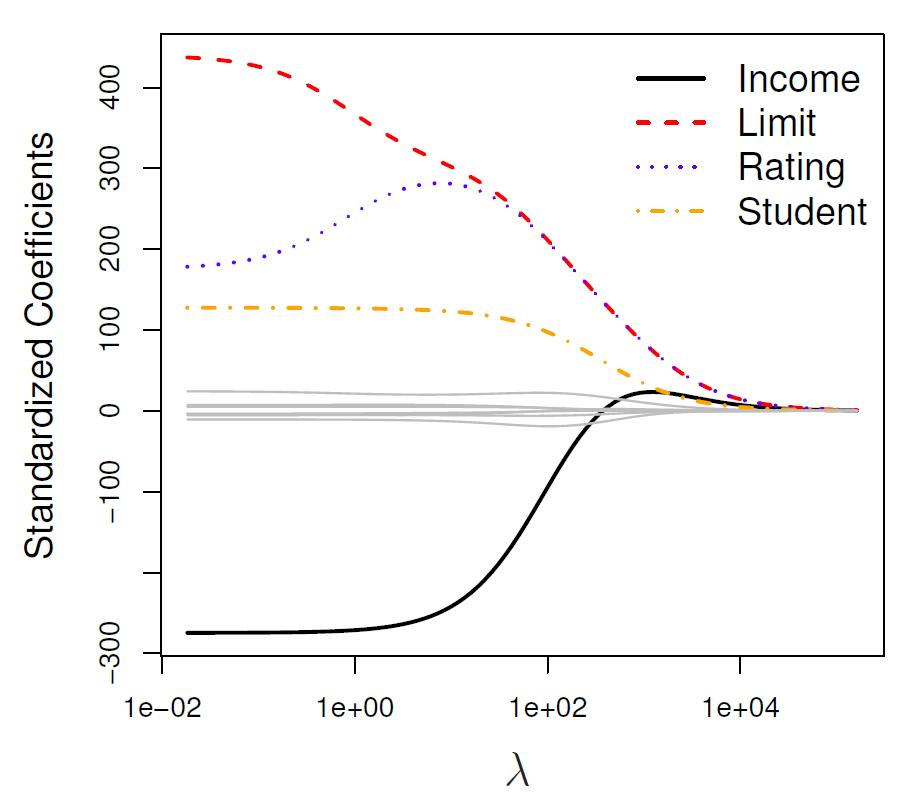
\includegraphics[scale=0.30]{IMG/Ridge.jpg}
\end{figure}
\vspace{-0.5cm}
\centering Coefficient estimates are plotted as a function of $\lambda$.
\end{frame}

%------------------------------------------------
\begin{frame}{Ridge regression}
\begin{itemize}
\item The standard OLS coefficient estimates are scale equivariant: multiplying $x_j$ by a constant $c$ simply leads to a scaling of the least squares coefficient estimates by a factor of $1/c$.\\ 
\medskip Regardless of predictor scaling, $ ( \hat{\beta}_j x_{ij} )$ will remain the same.
\medskip
\item In contrast, the ridge regression coefficient estimates can change substantially when multiplying a given predictor (or other predictors!) by a constant, due to the sum of squared coefficients term in the penalty part of the ridge regression objective function.
\medskip
\item Therefore, it is best to apply ridge regression after standardizing the predictors, using the formula:
$$ \widetilde{x}_{ij} = \frac{x_{ij}}{
   \sqrt[]{\frac{1}{n} \sum_{i=1}^n (x_{ij} - \overline{x}_j)^2 \,}}
   \quad \textnormal{hence} \quad
   \textnormal{s.d.}(\widetilde{x}_{j}) = 1\, ; \, j=1,2,\dots$$
 
\end{itemize}
\end{frame}
%------------------------------------------------
\begin{frame}{Ridge regression - final remarks}
$$\underset{\bm{\beta}}{\textnormal{min:~}} 
\left[ \sum_{i=1}^n \left(y_i - \hat{\beta}_0 
- \sum_{j=1}^p  \hat{\beta}_j x_{ij} \right)^2 
\! + \lambda \sum_{j=1}^p  \hat{\beta}_j^2 \right]
$$
\begin{itemize}
\item Ridge solutions are not equivariant under scaling of the inputs, 
\\so we standardize the inputs before estimation \\(this just recaps previous page).
\medskip
\item The intercept $\beta_0$ has been left out of the penalty term. Penalization of the intercept would make the procedure depend \\on the origin chosen for $y$.
\medskip
\item Ridge penalty shrinks coefficients towards zero (except $\hat{\beta}_0$). \\Coefficients of correlated variables are shrunk toward each other. \\ (See 
\textcolor{blue}{\underline{\href{https://web.stanford.edu/~hastie/ElemStatLearn/}{chapter 3 of ESLII}}} for detailed technical discussion.)
\end{itemize}
\end{frame}
%------------------------------------------------
\begin{frame}{Ridge regression - final remarks}
For LRM, RSS and OLS may be easily written in matrix form as:
\begin{itemize}
\item $\textit{RSS}(\textnormal{OLS}) = (\bm{y}-\bm{X\beta})^{\prime}(\bm{y}-\bm{X\beta})$
\item ~~~~~~~$\hat{\bm{\beta}}_{\textnormal{OLS}} = (\bm{X}^{\prime}\bm{X})^{-1}\bm{X}^{\prime}\bm{y}$ 
\end{itemize}
For ridge regression, this may be re-written as
\begin{itemize}
\item $\textit{RSS}(\lambda) = (\bm{y}-\bm{X\beta})^{\prime}(\bm{y}-\bm{X\beta}) 
+ \lambda \,\bm{\beta}^{\prime} \!\bm{\beta}$
\item ~~$\,\hat{\bm{\beta}}_{\textnormal{ridge}} = (\bm{X}^{\prime}\bm{X} + \lambda \bm{I}_p )^{-1}\bm{X}^{\prime}\bm{y}$ 
\end{itemize}

With the choice of quadratic penalty $\bm{\beta}^{\prime} \!\bm{\beta}$, the ridge regression solution is again a linear function of $y$. 

\medskip
Ridge method adds a positive constant to the diagonal of $(\bm{X}^{\prime}\bm{X})$ before inversion. This makes the problem non-singular, even if $(\bm{X}^{\prime}\bm{X})$ is not of full rank (perfect multicollinearity, $p>n$, $p \gg n$).

\medskip
This was the main motivation for ridge regression when it was first introduced in statistics (Hoerl and Kennard, 1970)

\end{frame}
%------------------------------------------------
\begin{frame}{Lasso regression}
\begin{itemize}
\item Ridge regression does have one obvious disadvantage:
unlike subset selection, which will generally select models
that involve just a subset of the variables, ridge regression
will include all $p$ predictors in the final model.
\medskip
\item The Lasso is a relatively recent alternative to ridge
regression that overcomes this disadvantage. The lasso
coefficients,  $\bm{\hat{\beta}}_{\!L}$ estimates 
are the values that minimize the penalized RSS:
$$
\underset{\bm{\beta}}{\textnormal{min:~}} 
\left[
\sum_{i=1}^n \left(y_i - \hat{\beta}_0 
- \sum_{j=1}^p  \hat{\beta}_j x_{ij} \right)^2 
\! + \lambda \sum_{j=1}^p  | \hat{\beta}_j | \right]$$
again, $\lambda > 0$ is a tuning parameter, determined separately ($k$FCV).
\item In statistical parlance, the lasso uses an $\ell_1$ (pronounced ``ell 1'') penalty instead of an $\ell_2$ penalty. The $\ell_1$ norm of a coefficient vector  is given by 
$\| \beta \|_1 = \sum | \beta |$.
\end{itemize}
\end{frame}
%------------------------------------------------
\begin{frame}{Lasso regression - example}
\vspace{-1cm}
\begin{figure}
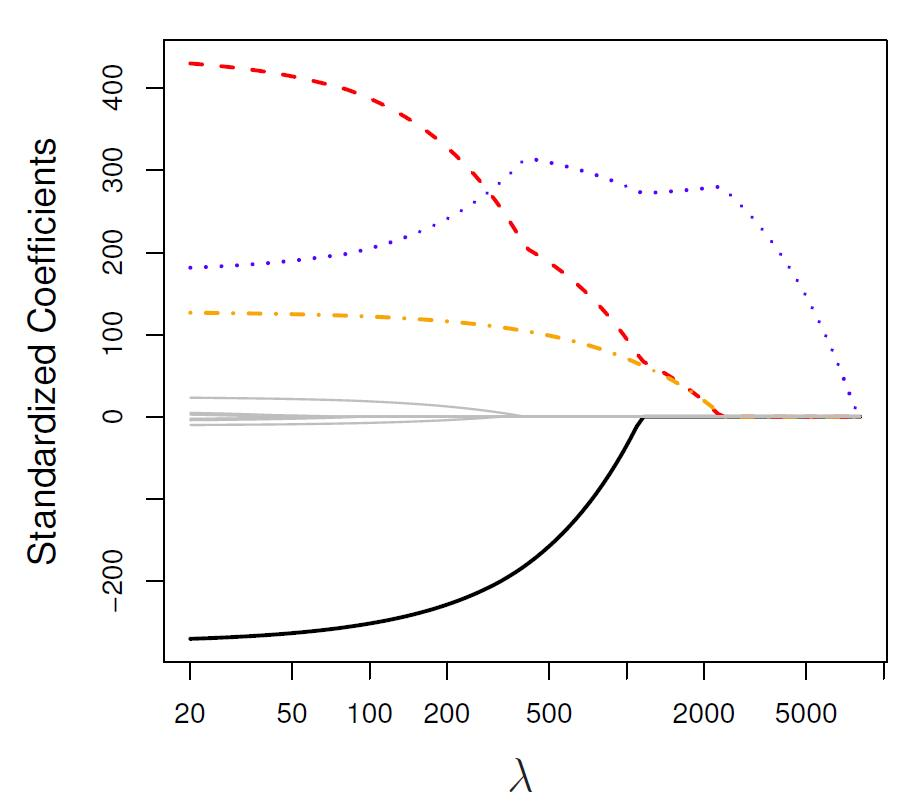
\includegraphics[scale=0.30]{IMG/Lasso.jpg}
\end{figure}
\vspace{-0.5cm}
\centering Coefficient estimates are plotted as a function of $\lambda$.
\end{frame}
%------------------------------------------------
\begin{frame}{Lasso regression}
\begin{itemize}
\item As with ridge regression, the lasso shrinks the coefficient
estimates towards zero.
\medskip
\item In the case of the lasso, the $\ell_1$ penalty has the
effect of forcing some of the coefficient estimates to be
exactly equal to zero when the tuning parameter $\lambda$ is
sufficiently large (see \textcolor{blue}{\underline{\href{http://www-bcf.usc.edu/~gareth/ISL/}{ISLR textbook}}}).
\medskip
\item Much like stepwise model selection, the lasso regression performs variable selection.
\medskip
\item Lasso yields sparse models - that is, models that involve only \\a subset of the variables.
\medskip
\item As in ridge regression, selecting a good value of $\lambda$ for the
lasso is critical; cross-validation is used.
\end{itemize}
\end{frame}
%------------------------------------------------
\begin{frame}{Ridge \& Lasso - discussion}
\begin{itemize}
\item Neither ridge regression nor the lasso will universally dominate the other.
\medskip
\item In general, one might expect the lasso to perform better
when the response is a function of only a relatively small
number of predictors.
\medskip
\item However, the number of predictors that is related to the
response is never known a priori for real data sets.
\medskip
\item CV can be used in order to determine which approach is better on a particular data set.
\end{itemize}
\end{frame}
%------------------------------------------------
\begin{frame}{Ridge \& Lasso - $\lambda$ selection}
Cross-validation is used to determine $\lambda$, as follows:
\bigskip
\begin{enumerate}
\item We choose a grid of $\lambda$ values and compute the
cross-validation error rate for each value of $\lambda$.
\medskip
\item We select the tuning parameter $\lambda$, for which the
cross-validation error is smallest.
\medskip
\item Finally, the model is re-fit using all of the available
observations and the selected value of the tuning
parameter $\lambda$.
\end{enumerate}
\bigskip
The above steps 1 and 2 can be performed for both ridge and lasso.\\
~~\dots cross-validation errors are compared to select ``best'' $\lambda$ \\
~~\dots and to choose between ridge and lasso.

\end{frame}
%------------------------------------------------
\begin{frame}{Elastic net regression (penalty)}
$$\min \left[ \sum_{i=1}^n \left(y_i - \hat{\beta}_0 
         - \sum_{j=1}^p  \hat{\beta}_j x_{ij} \right)^2 
         \! + \lambda \sum_{j=1}^p 
         \left( \alpha |\beta_j| + (1-\alpha) \hat{\beta}_j^2 \right) \right]
$$
\begin{itemize}
\item \textbf{Lasso penalty} encourages sparse solutions (in terms of coefficients), yet it is somewhat indifferent to the choice among a set of strong but correlated regressors.
\smallskip
\item \textbf{Ridge penalty} shrinks coefficients of correlated variables toward each other, no spare solution effect.
\smallskip
\item \textbf{Elastic net penalty} is a compromise (combined method). The second term of the penalization element encourages highly correlated features to be averaged, while
the first term encourages a sparse solution in the coefficients of these averaged features.
\end{itemize}
\end{frame}
%------------------------------------------------
\begin{frame}{Elastic net regression (penalty)}
$$\min \left[ \sum_{i=1}^n \left(y_i - \hat{\beta}_0 
         - \sum_{j=1}^p  \hat{\beta}_j x_{ij} \right)^2 
         \! + \lambda \sum_{j=1}^p 
         \left( \alpha |\beta_j| + (1-\alpha) \hat{\beta}_j^2 \right) \right]
$$
\begin{itemize}
\item The elastic net penalty can be used with any linear model \\(LM, GLM), in particular for regression or classification.\\
Logit (GLM/MLE) example of elastic net penalty generalization:\\
\footnotesize{$\underset{\bm{\beta}}{\textnormal{max}}\!
\left[
\sum_{i=1}^n \!\left( y_i \log [G(\bm{x}_i\bm{\beta})] \!+\! 
(1\!-\!y_i) \log [1\!-\!G(\bm{x}_i\bm{\beta})]
\right)
- \lambda \sum_{j=1}^p \!\left( \alpha |\beta_j|\!+\!(1\!-\!\alpha) \hat{\beta}_j^2 \right)
\right]$}
\smallskip
\normalsize{
\item Parameter $\alpha$ determines the relative mix of ridge and lasso penalties. It is set prior to model estimation.
\medskip
\item CV can be used to chose $\alpha$ and $\lambda$.}
\end{itemize}
\end{frame}
%------------------------------------------------
\subsection{Dimension reduction: PCR \& PLS}
\begin{frame}{High dimensionality \& dimension reduction methods}
\end{frame}
%------------------------------------------------
\begin{frame}{Principal component vs. Factor analysis}
\textbf{PCA vs FA -- quick overview:}\\
\medskip
\begin{itemize}
\item \textbf{Principal component analysis} involves extracting linear composites of observed variables. We use PCA to reduce \\a dataset of correlated observed variables to a smaller set of important independent composite variables.
\bigskip
\item \textbf{Factor analysis} is based on a formal model predicting observed variables from theoretical latent factors. We use FA for testing/estimating a theoretical model of latent factors causing observed variables.
\end{itemize}
\bigskip
The following discussion uses PCA-based approach.
\end{frame}
%------------------------------------------------
\begin{frame}{Dimension reduction methods}
\begin{itemize}
\item Stepwise regression, ridge and lasso involve fitting linear regression models (by OLS or by parameter shrinkage) using the original predictors: $x_1, x_2, \dots , x_p$.
\medskip
\item \textbf{Dimension reduction methods} transform the
predictors and then fit a least squares model using the
transformed variables:
\begin{enumerate}
\bigskip
\item \textbf{Principal components analysis (PCA)}: data (pre)processing, \textcolor{blue}{\textbf{feature extraction -- dimension reduction with minimized information loss.}} PCA output can be used in supervised methods of analysis (OLS).
\bigskip
\item \textbf{Principal component regression (PCR)}:  In the LRM, the potentially many correlated original variables are replaced with a small set of principal components that capture their joint variation.
\end{enumerate}
\end{itemize}
\end{frame}
%------------------------------------------------
\begin{frame}{Principal component analysis (PCA)}
\begin{itemize}
\item PCA produces a low-dimensional representation of a dataset. It finds a sequence of linear combinations of the variables that have maximal variance and are mutually uncorrelated.
\medskip
\item Apart from producing derived variables for use in supervised learning problems, PCA also serves as a tool for data visualization.
\medskip
\item Suppose we have a $(n \! \times \! p)$ dataset $\bm{X}$. Since we are mainly interested in variance here, we can assume that each of the variables in $\bm{X}$ has been \textbf{centered} to have mean zero \\(all column-means of $\bm{X}$ are zero). If necessary, the transformation (centering of $\bm{X}$) is straight-forward.
\medskip
\item Typically, empirical analyses (in \texttt{R} and elsewhere) would involve variable standardizing/scaling to $\textnormal{var}(\bm{x}_j)=1$.
\end{itemize}
\end{frame}
%---------------------------------------------------------------------
\begin{frame}{PCA motivation \& example}
\vspace{-0.3cm}
\begin{figure}
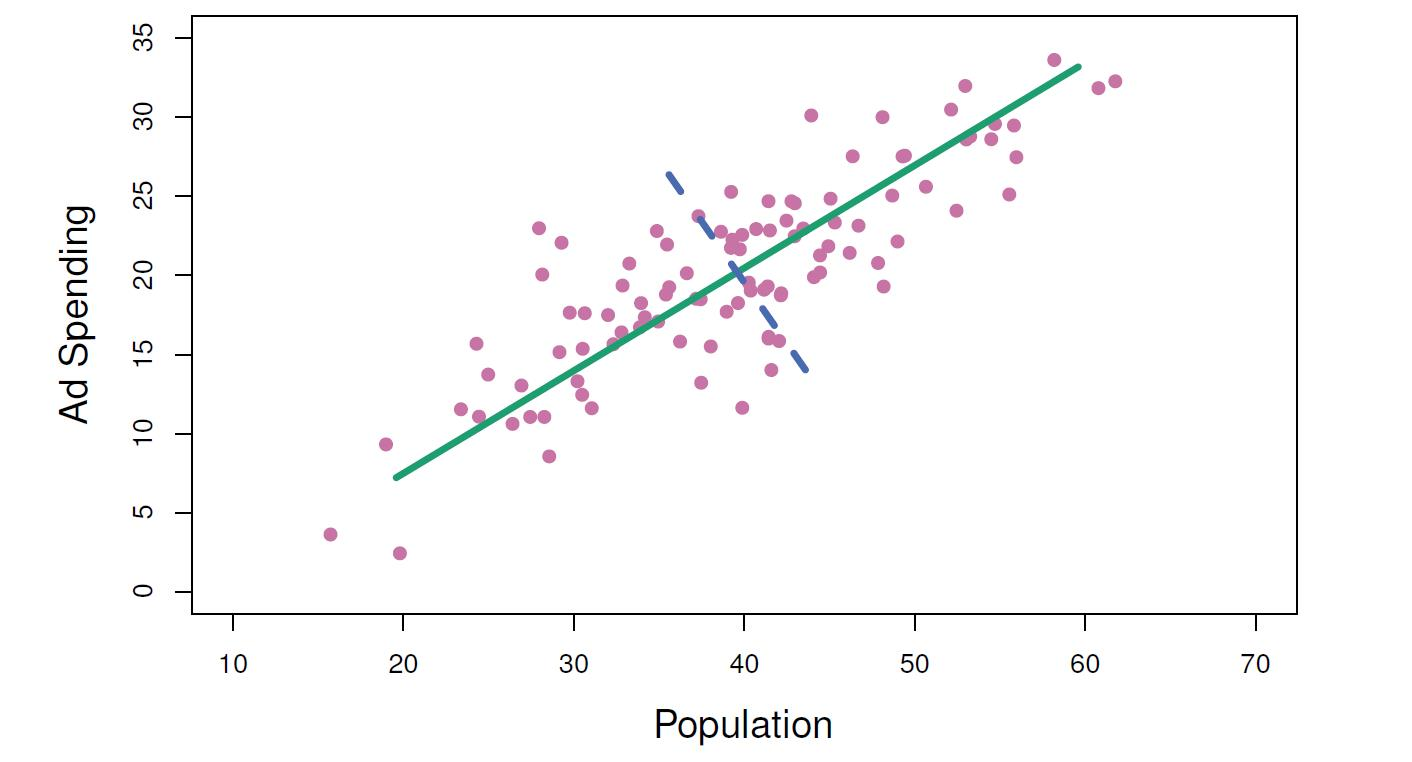
\includegraphics[scale=0.30]{IMG/PCAexample.jpg}
\end{figure}
\vspace{-0.3cm}
\centering Sample dataset with 2 variables. Green line indicates the first principal component, $Z_1$. Along $Z_1$, data varies the most (out of all directions possible -- in 2D). Blue dashed line indicates $Z_2$ (most variability orthogonal to $Z_1$).
\end{frame}
%---------------------------------------------------------------------
\begin{frame}{PCA motivation \& example}
\vspace{-1.0cm}
\begin{figure}
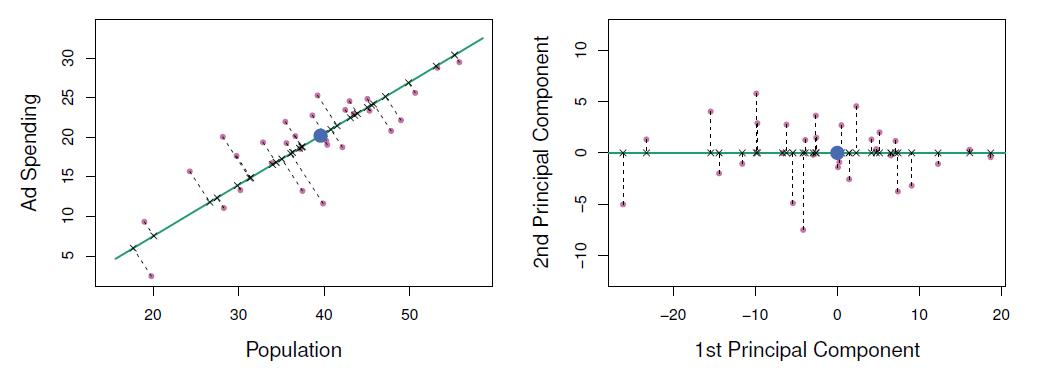
\includegraphics[scale=0.42]{IMG/PCAexample2.jpg}
\end{figure}
\vspace{-0.1cm}
\centering Sample dataset with 2 variables.  \\$Z_1$ minimizes the squared perpendicular distances to observed data. Data vary most along $Z_1$ (data most spread-out along $Z_1$). \\Values of $z_{i1} \in Z_1$ and $z_{i2} \in Z_2$ are shown as distances from ``zero'' (blue dot). Right panel/plot is rotated for readability.
\end{frame}
%---------------------------------------------------------------------
\begin{frame}{PCA motivation \& example}
\vspace{-2.2cm}
\begin{figure}
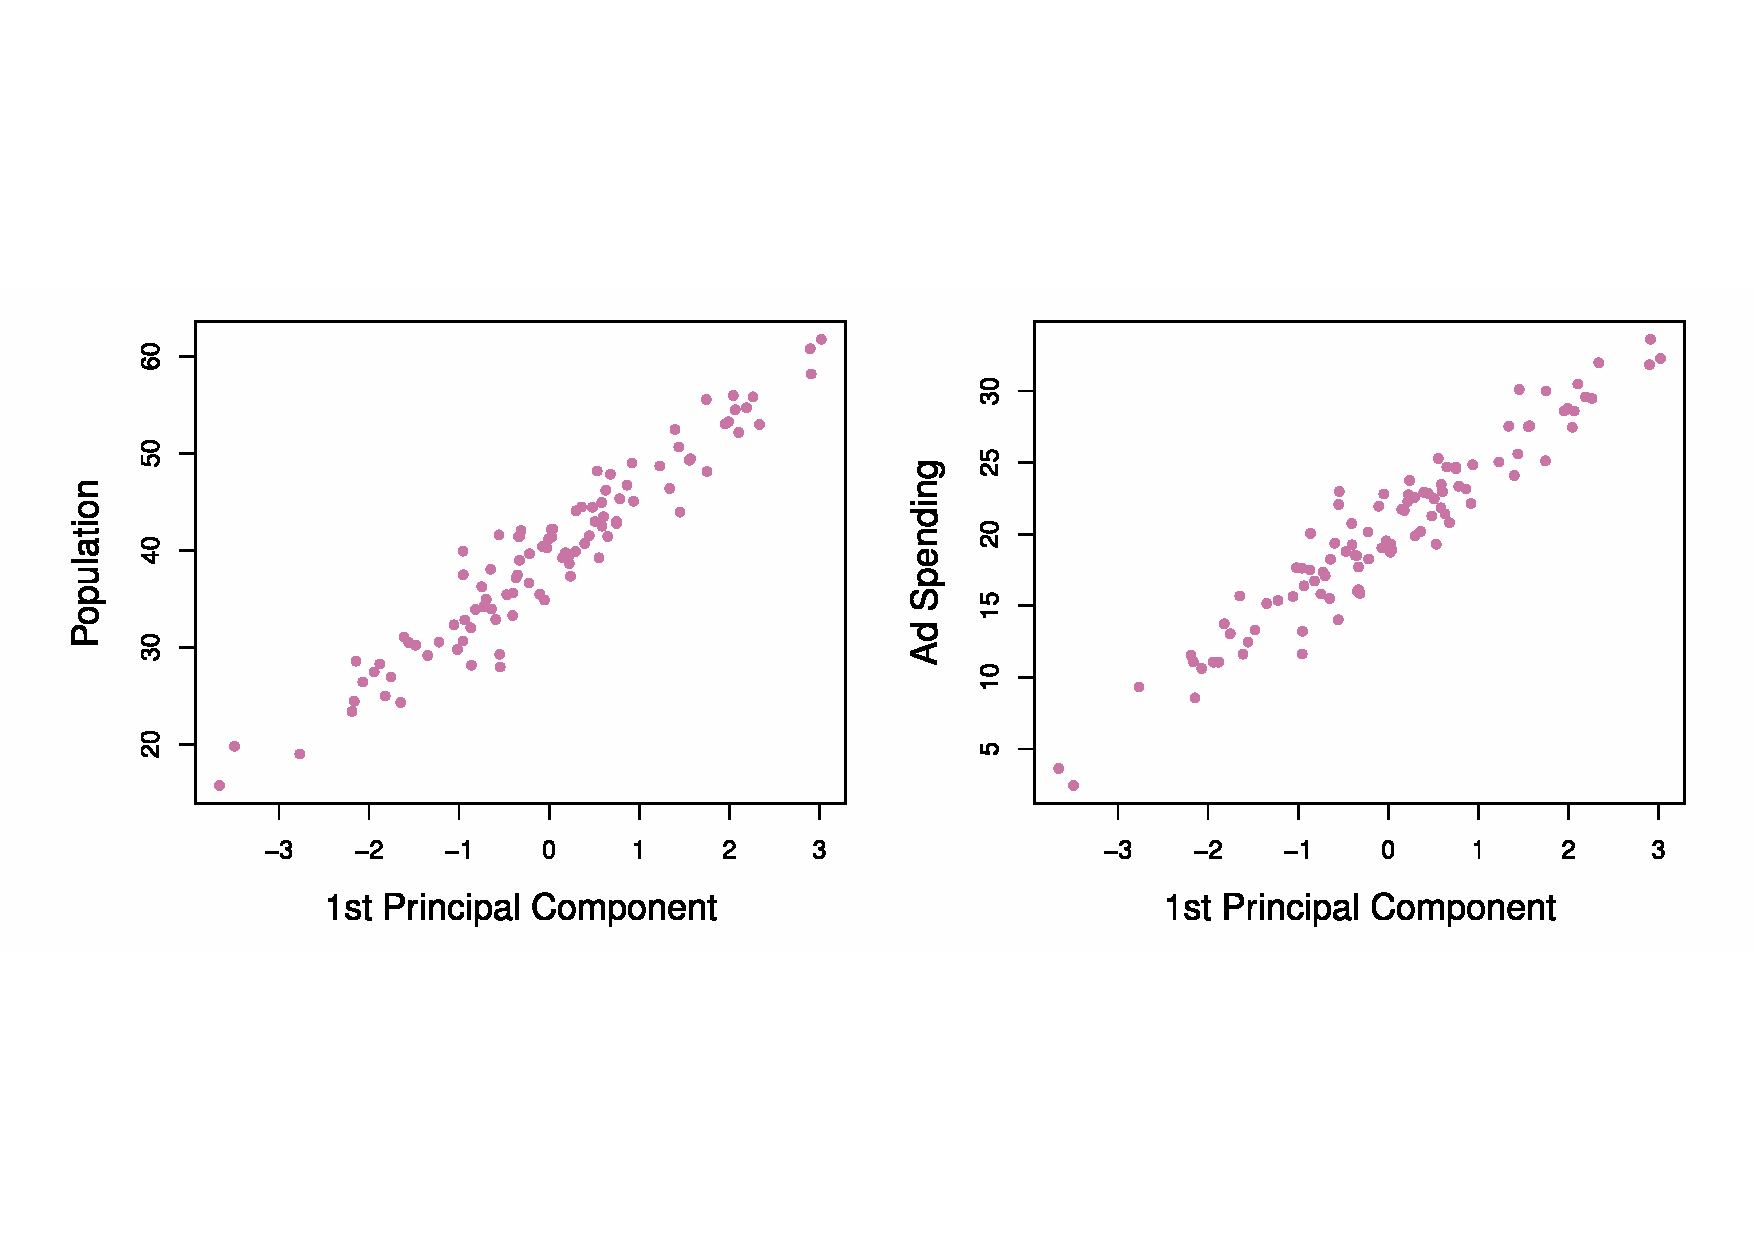
\includegraphics[scale=0.40]{IMG/PCAExample3.pdf}
\end{figure}
\vspace{-2cm}
\centering Sample dataset with 2 variables. First principal component is shown (on the $x$-axis) against \texttt{Population} and \texttt{Ad Spending} variables. \\Strong correlation is apparent in both plots, $ \rightarrow ~Z_1$ summarizes both series well and can be used as a single composite predictor for \texttt{Sales} \\(instead of the two observed regressors).
\end{frame}
%---------------------------------------------------------------------
\begin{frame}{PCA motivation \& example}
\vspace{-2.2cm}
\begin{figure}
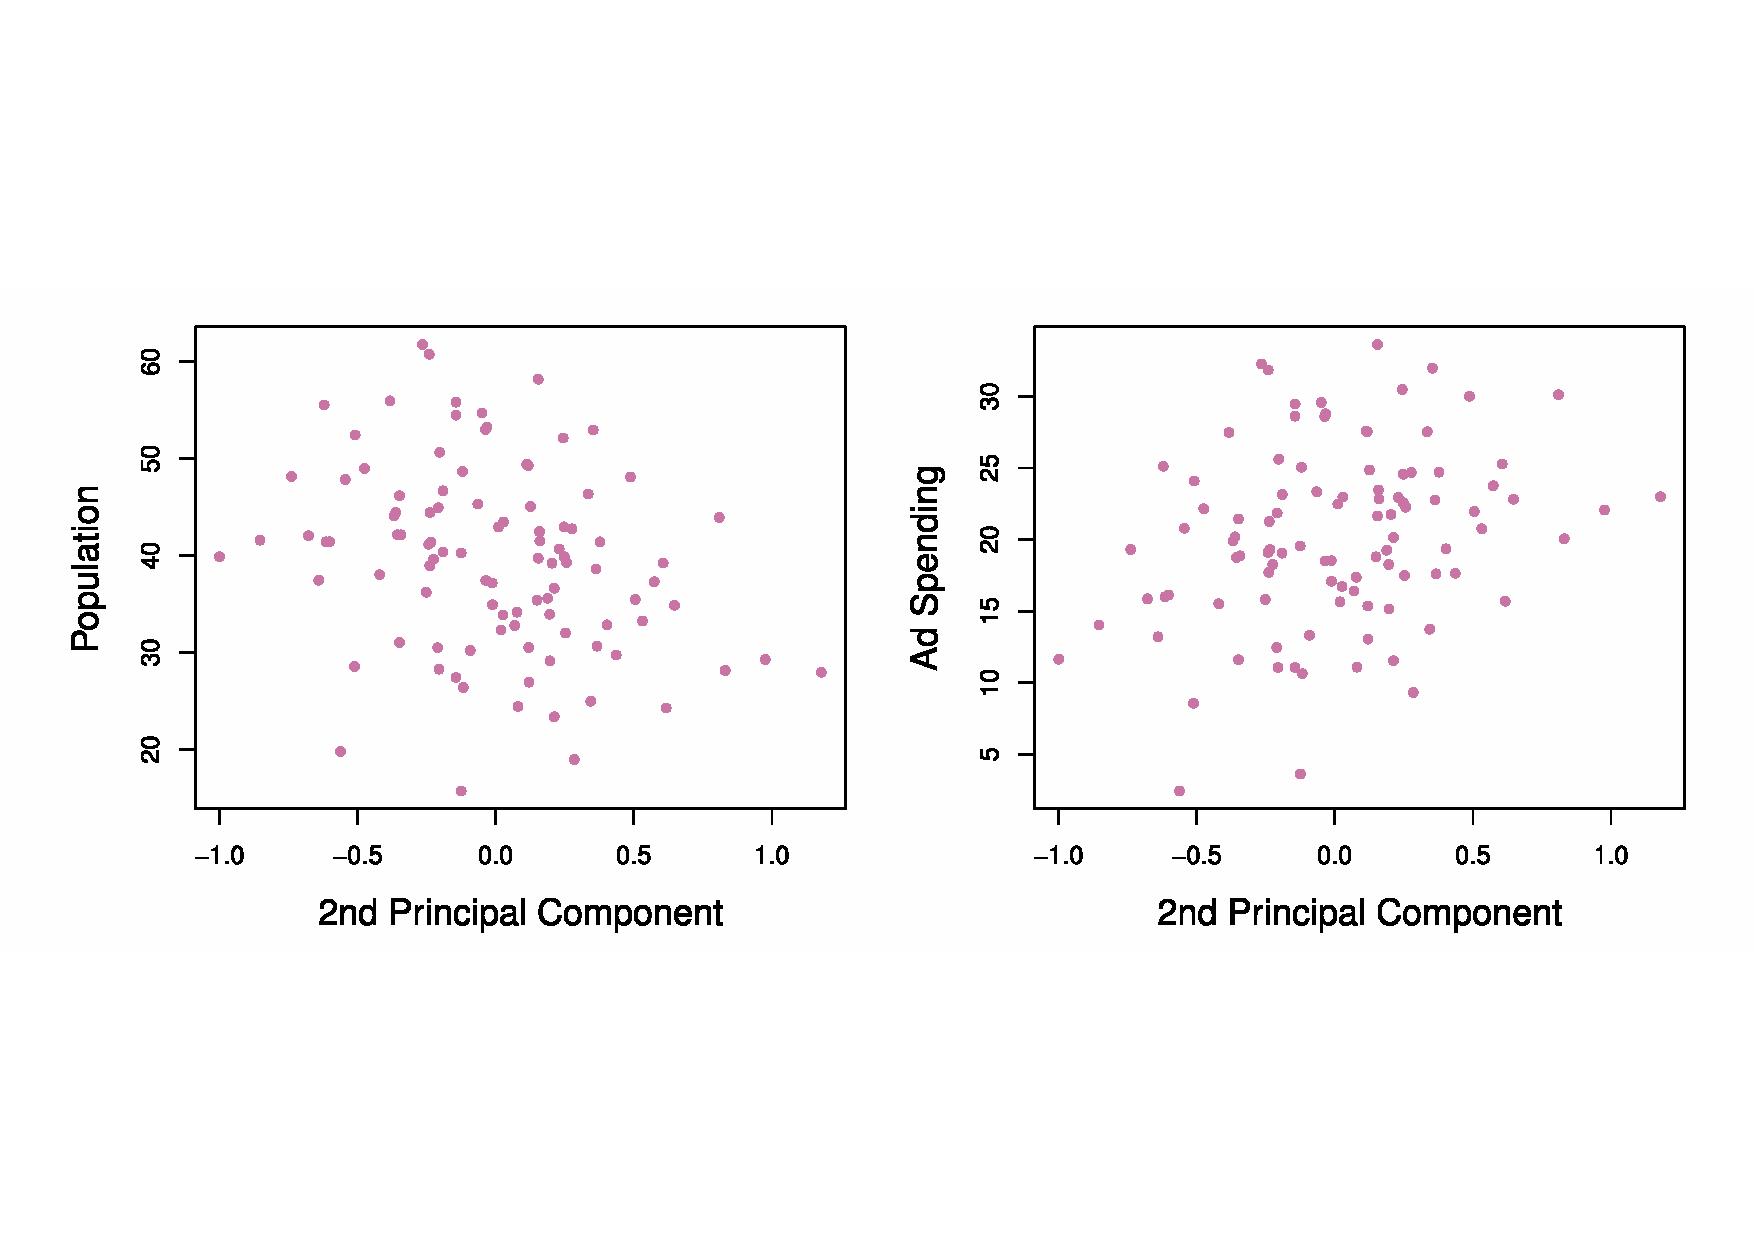
\includegraphics[scale=0.40]{IMG/PCAExample4.pdf}
\end{figure}
\vspace{-2cm}
\centering Sample dataset with 2 variables. Second principal component is shown (on the $x$-axis) against \texttt{Population} and \texttt{Ad Spending} variables. \\There is little relationship between $Z_2$ and the two regressors. \\Hence, $Z_1$ apparently summarizes both (strongly correlated) regressors well enough. 
\end{frame}
%---------------------------------------------------------------------
\begin{frame}{Principal component analysis (PCA)}
\begin{itemize}
\item $1^{\textnormal{st}}$ principal component vector $\bm{z}_1$ of a set of centered variables
$\bm{x}_1, \bm{x}_2, \dots, \bm{x}_p$ (all $n\!\times\!1)$ is the normalized linear combination:
\vspace{-0.1cm}
$$ \bm{z}_1 = \phi_{11}\bm{x}_1 + \phi_{21}\bm{x}_2 + \dots + \phi_{p1}\bm{x}_p$$
\vspace{-0.1cm}
that has the largest variance. Hence, we solve:
\begin{equation} \label{PCA1}
\underset{\phi_{11},\dots,\phi_{p1}}{\textnormal{maximize}} \, 
  \frac{1}{n} \sum_{i=1}^n \left( \sum_{j=1}^p  
  \phi_{j1}x_{ij} \right)^{\!2} \,\,\,\,\,\, s.\,t. \,\,\,\,\,\,     
  \sum_{j=1}^p \phi_{j1}^2=1 
\end{equation}
\item The $\phi_{j1}$ elements $\phi_{11}, \dots, \phi_{p1}$ are \textit{loadings} of the first principal component and they make up the first principal component loading vector, $\bm{\phi}_1 = (\phi_{11}, \phi_{21},\dots, \phi_{p1})^\prime$.
\item $\sum_{j=1}^p \phi_{j1}^2 =1$ is the normalization condition: sum of squares of loadings is equal to one. Otherwise, setting $|\phi_{j1}|$ arbitrarily large leads to arbitrarily large variance.
\item \eqref{PCA1} is solvable by linear algebra (singular-value decomposition)
\end{itemize}
\end{frame}
%---------------------------------------------------------------------
\begin{frame}{Principal component analysis (PCA)}
\begin{itemize}
\item By solving \eqref{PCA1}, we obtain the linear combination of the sample variables of the form:
$$z_{i1}= \phi_{11}x_{i1} + \phi_{21}x_{i2} + \dots + \phi_{p1}x_{ip} \,\,\,\,\,\,;\,\,\,\,\,\,            i=1,\dots,n.$$
\item $\bm{z}_1 = (z_{11}, z_{21}, \dots, z_{n1})^{\prime}$ is the first principal component. 
\medskip
\item Since each of the $\bm{x}_j$ variables has mean zero, so does $\bm{z}_1$\\~\\
Hence, the sample variance of $\bm{z}_1$ can be calculated as $\frac{1}{n} \sum_{i=1}^n z_{i1}^2$.
\end{itemize}
\end{frame}
%---------------------------------------------------------------------
\begin{frame}{Principal component analysis (PCA)}
\begin{itemize}
\item The loading vector $\bm{\phi}_1$ with elements $\phi_{11}, \phi_{21},\dots, \phi_{p1}$ defines a direction in variable space (column space of $\bm{X}$), along which the data vary the most.
\medskip
\item \textbf{The second principal component} is the linear combination
of $\bm{x}_1, \dots , \bm{x}_p$ that maximizes variance among all linear combinations that are \textbf{uncorrelated} with $\bm{z}_1$. Hence, we add orthogonality condition to \eqref{PCA1} and repeat the optimization.
\medskip
\item The second principal component $\bm{z}_2$ and its elements $z_{12}, z_{22}, \dots z_{n2}$ take the form:
$$z_{i2}= \phi_{12}x_{i1} + \phi_{22}x_{i2} + \dots + \phi_{p2}x_{ip} \,\,\,\,\,\,;\,\,\,\,\,\,            i=1,\dots,n.$$
where $\bm{\phi}_2 = (\phi_{12}, \phi_{22},\dots, \phi_{p2})^\prime$ is the second principal component loading vector.
\end{itemize}
\end{frame}
%----------------------------------------------------------------------
\begin{frame}{Principal component analysis (PCA)}
\begin{itemize}
\item Constraining $\bm{z}_2$ to be uncorrelated with $\bm{z}_1$ is equivalent to constraining the direction $\bm{\phi}_2$ to be orthogonal (perpendicular) to the direction $\bm{\phi}_1$. 
\medskip
\item Subsequent principal components: \\ \medskip For a sequence of additional $\bm{z}_2, \bm{z}_3,\dots$ principal components, we solve \eqref{PCA1} while adding orthogonality condition with respect to all preceding principal components.
\medskip
\item Important geometrical interpretations to principal components apply (see \textcolor{blue}{\underline{\href{http://www-bcf.usc.edu/~gareth/ISL/}{ISLR textbook}}}).
\end{itemize}
\end{frame}
%---------------------------------------------------------------------
\begin{frame}{Principal component analysis (PCA)}
\textbf{Proportion of variance explained by principal components}\\
\begin{itemize}
\item To understand the ``strength'' of each principal component, we calculate the proportion of variance explained by each component.
\medskip
\item \textbf{Total variance present in a data set} (assuming $\bm{X}$ matrix ($n\!\times\!p)$ of centered variables $\bm{x}_j$ with mean zero) is defined as:
$$ \sum_{j=1}^p \textnormal{var}\,(\bm{x}_j) 
   = \sum_{j=1}^p \frac{1}{n} \sum_{i=1}^n x_{ij}^2 $$
\item \textbf{Variance explained} by the $m$-th principal component is:
$$ \textnormal{var}\,(\bm{z}_m) 
   = \frac{1}{n} \sum_{i=1}^n z_{im}^2 $$
\item $\sum_{j=1}^p \textnormal{var}\,(\bm{x}_j) = \sum_{m=1}^M \textnormal{var}\,(\bm{z}_m), $  where $M = \min(n-1, p)$. \\i.e. if all PC are used, they explain 100 \% of variance in $\bm{X}$.
\end{itemize}
\end{frame}
%---------------------------------------------------------------------
\begin{frame}{Principal component analysis (PCA)}
\textbf{Proportion of variance explained (PVE)}\\
\bigskip
\begin{itemize}
\item PVE of the $m$-th principal component $\bm{z}_m$ lies between 0 and 1 and it is defined as:
$$\textnormal{PVE}_m 
 = \frac{\sum_{i=1}^n z_{im}^2 }
 {\sum_{j=1}^p \sum_{i=1}^n x_{ij}^2}  \,.$$\\
\bigskip
\item Also, $$\sum_{m=1}^M \textnormal{PVE}_m = 1~,~~$$ \\~\\i.e. PVEs sum to 1 and we can display \& interpret cumulative PVEs.
\end{itemize}
\end{frame}
%---------------------------------------------------------------------
\begin{frame}{Principal component analysis (PCA)}
\texttt{R} example:\\
\smallskip
\footnotesize{
\texttt{pca1 = princomp(x, scores=TRUE, cor=TRUE) \# x has 7 columns\\
summary(pca1)\\
~\\
\#\# Importance of components:\\
\#\# ~~~~~~~~~~~~~~~~~~~~~~~~~~Comp.1~~~~~Comp.2~~~~~Comp.3~~~~~~Comp.4\\
\#\# Standard deviation~~~~~1.9036937~ 1.0423367~ 0.81837919~ 0.75632747\\
\#\# Proportion of Variance 0.5177214~ 0.1552094~ 0.09567779~ 0.08171875\\
\#\# Cumulative Proportion~ 0.5177214~ 0.6729308~ 0.76860854~ 0.85032729\\
\#\# ~~~~~~~~~~~~~~~~~~~~~~~~~~Comp.5~~~~~~Comp.6~~~~~~Comp.7\\
\#\# Standard deviation~~~~~0.64958592~ 0.56978592~ 0.54871770\\
\#\# Proportion of Variance 0.06028027~ 0.04637943~ 0.04301302\\
\#\# Cumulative Proportion~ 0.91060756~ 0.95698698~ 1.00000000\\
}
\begin{itemize}
\item The number of components is also the number of variables (if $n>p$).
\item Proportion of variance: Eg. if $\textnormal{PVE}_1 = .52$, $\bm{z}_1$ explains 52\% of variance in $\bm{X}$.
\item Cumulative Proportion: PVE by $\bm{z}_m$ and previous components.
\item Standard deviation = eigenvalues
\item How many components to use in PCR? Choose the components with eigenvalues equal or higher than 1. (or use cross-validation)
\end{itemize}
}
\end{frame}
%---------------------------------------------------------------------
\begin{frame}{Kaiser-Meyer-Olkin (KMO) statistic}
PCA can perform a compression of the available information (reduce dimension) only if we can ``reject''  independence (orthogonality) among variables $\bm{x}_j$ in $\bm{X}$.
\bigskip
Individual $\textit{KMO}$ (for $j$-th variable):
$$\textit{KMO}_j = \frac{\sum_{i\neq j} r_{ij}^2}{\sum_{i\neq j} r_{ij}^2 + \sum_{i\neq j} a_{ij}^2}\,;\hspace{1,7cm} \textit{KMO}_j \in \langle 0,1 \rangle $$\\
Overall $\textit{KMO}$:
$$\textit{KMO} = \frac{\sum_j \sum_{i\neq j} r_{ij}^2}
                   {\sum_j \sum_{i\neq j} r_{ij}^2 \,+\, \sum_j \sum_{i\neq j} a_{ij}^2}\,
                   ;\hspace{0.5cm} \textit{KMO} \in \langle 0,1 \rangle $$\\

where:\\
$\{r_{ij} \} = \bm{R}$, which is a correlation matrix (here, $i$, $j$ denote variables),\\
$\{a_{ij} \} = \bm{A}$, which is a partial correlation matrix (partial correlations represent the direct interactions between two variables, with the indirect effects of all remaining variables removed)\\
$a_{ij} = - \frac{v_{ij}}{\sqrt[]{v_{ii} \cdot v_{jj}\,}}$ where $\{ v_{ij} \} = \bm{V} = \bm{R}^{-1}$
\end{frame}
%------------------------------------------------
\begin{frame}{Kaiser-Meyer-Olkin (KMO) statistic}
$\textit{KMO}$ description 
\begin{itemize}
\item $\textit{KMO}$ compares  correlations between variables against their partial correlations. 
\item If partial correlations $a_{ij}$ are near zero, PCA can perform efficiently, because the
variables are highly related and $\textit{KMO} \approx 1$.
\item If $\textit{KMO}$ is low (KMO $\approx 0$), PCA is not relevant.\\In empirical applications, PCA is gerally not usefull if $\textit{KMO} < 0.5$.
\end{itemize}
\bigskip
$\textit{KMO}$-based variable selection:
\smallskip
\begin{itemize}
\item Overall $\textit{KMO}$ should be .60 or higher (ideally over 0.90).
\item If it is not, drop the variables with the lowest individual $\textit{KMO}_j$ values, until overall $\textit{KMO}$ rises above .60.
\item This approach requires that we start with multiple variables/regressors in our dataset; at least $p > 5$ .
\item Alternative: Bartlett’s test in \texttt{R}: cortest.bartlett() in \{psych\}.
\end{itemize}
\end{frame}
%------------------------------------------------
\begin{frame}{Principal component regression (PCR)}
\textbf{PCR motivation:}\\
\bigskip
If we have many correlated original variables as regressors in a LRM, we can replace them with a small set of principal components that capture their joint variation.
\medskip
\begin{itemize}
\item Variance-Bias tradeoff benefits
\item Models unsuitable for LRM-like parameter interpretation
\end{itemize}
\end{frame}
%------------------------------------------------
\begin{frame}{Principal component regression (PCR)}
\begin{itemize}
\item Using PCA, we linearly transform our dataset of predictors $\bm{x}_1, \bm{x}_2, \dots, \bm{x}_p$ into $\bm{z}_1, \bm{z}_2, \dots, \bm{z}_M$ variables where $M < p$. \\The PCA transformation can be outlined as follows: 
\begin{equation} \label{PCR1}
\bm{z}_m = \bm{X\phi}_m \qquad \textnormal{where} \qquad z_{im} = \sum_{j=1}^p \phi_{jm\,} x_{ij},
\end{equation}
for some constant parameters $\phi_{m1}, \dots, \phi_{mp}$.
\item Now, we can use OLS to fit a LRM:
\begin{equation} \label{PCR2}
y_i = \theta_0 + \sum_{j=1}^M \theta_m z_{im} + \varepsilon_i,
\end{equation}
\item Note that in model \eqref{PCR2}, the regression coefficients are given
as $\theta_0, \dots, \theta_M$. If the constants $\phi_{1m}, \phi_{2m}, \dots , \phi_{pm}$ are chosen wisely (PCA), then such dimension reduction approaches can often
outperform OLS regression in terms of CV errors, etc.
\end{itemize}
\end{frame}
%------------------------------------------------
\begin{frame}{Principal component regression (PCR)}
From equation/definition \eqref{PCR1}, we can write
$$ \sum_{m=1}^M \theta_m z_{im} 
= \sum_{m=1}^M \theta_m \sum_{j=1}^p \phi_{jm} x_{ij} 
= \sum_{j=1}^p \sum_{m=1}^M \theta_m \phi_{jm} x_{ij} 
= \sum_{j=1}^p \beta_j x_{ij} 
$$ 
where 
\begin{equation} \label{PCR3}
\beta_j = \sum_{m=1}^M \theta_m \phi_{jm}.
\end{equation}
\begin{itemize}
\item Therefore, model \eqref{PCR2} can be thought of as a special case of the original linear regression model.
\item Dimension reduction serves to constrain the estimated $\beta_j$ coefficients, since now they must take the form \eqref{PCR3}.
\item This approach can have significant benefits in terms of bias-variance tradeoff.
\end{itemize}
\end{frame}
%------------------------------------------------
\begin{frame}{Principal component regression (PCR)}
PCR: algorithm
\begin{itemize}
\medskip
\item First, we apply principal components analysis (PCA) to find suitable linear combinations of predictors for use in our regression.
\medskip
\begin{itemize}
    \item The first principal component is the (normalized) linear
combination of the regressors that has the largest variance.
\medskip 
\item The second principal component has largest variance,
subject to being uncorrelated with the first.
\medskip
\item And so on. 
\end{itemize}
\medskip
\item The dependent variable is then regressed on few principal components, rather than many original regressors.\\ \medskip
The optimal number of principal components can be assessed using cross validation.
\end{itemize}
\bigskip
\end{frame}
%------------------------------------------------
\begin{frame}{Principal component regression (PCR)}
\vspace{-0.7cm}
\begin{figure}
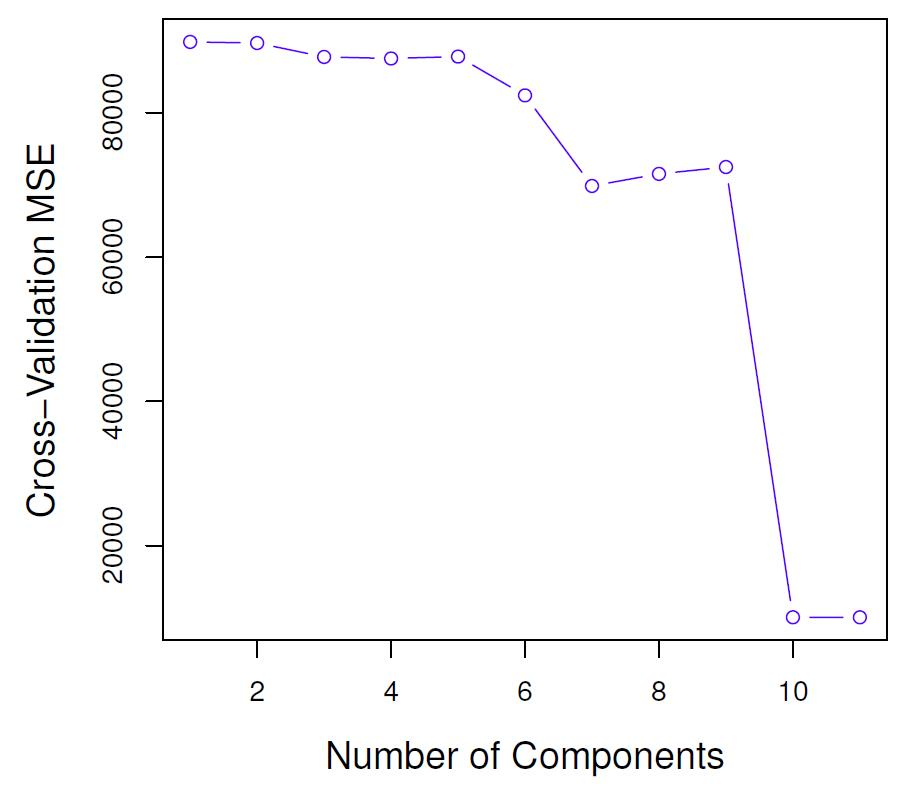
\includegraphics[scale=0.30]{IMG/PCRcomponent.jpg}
\end{figure}
\vspace{-0.5cm}
\centering Sample data, selection of the number of components. \\In this particular illustration, PCR would provide little improvement over OLS (this may happen often for $n\gg p$ datasets). 
\end{frame}
%------------------------------------------------
\begin{frame}{Principal component regression (PCR)}
\textbf{PCR: final discussion}
\medskip
\begin{itemize}
\item PCA identifies linear combinations (directions) that best
represent the predictors $\bm{x}_1, \bm{x}_2, \dots , \bm{x}_p$.
\item These directions are identified in an \textbf{unsupervised} way, since the response $y$ is not used to help determine the principal component directions. i.e. the response does not supervise the identification of the principal components.
\item PCR suffers from a potentially serious drawback: there is no guarantee that the directions that best explain the predictors will also be the best directions to use for predicting the response.
\end{itemize}
\medskip
Potential solutions to the problem:
\begin{itemize}
\item Partial least squares (\textcolor{blue}{\underline{\href{http://www-bcf.usc.edu/~gareth/ISL/}{ISLR, ch. 6.3.2}}})
\end{itemize}
\end{frame}
%---------------------------------------------------------------------
\begin{frame}{Partial least squares (PLS)}
\end{frame}
%---------------------------------------------------------------------
\begin{frame}{Partial least squares (PLS)}
\begin{itemize}
\item Much like with the PCR method, in PLS we also search for convenient (aggregating) linear combinations of regressors in matrix $\bm{X}$.\\
\medskip
\item PLS is not scale-invariant, so we assume each $\bm{x}_j$ regressor is standardized -- much the same way as in PCR.\\
\medskip
\item PLS, unlike PCR, uses \textit{supervised} identification of the components: both $\bm{X}$ and $\bm{y}$ are used when searching for linear combinations of regressors.\\
\medskip
\item PLS-based linear combinations of $\bm{x}_j$ (``directions'') not only approximate the original (correlated) data in $\bm{X},$ but are also related to the response $\bm{y}$.
\end{itemize}
\end{frame}
%---------------------------------------------------------------------
\begin{frame}{Partial least squares (PLS)}
First component for PLS:

$$ \bm{z}_1^{\textnormal{PLS}} = \bm{X\psi}_1 \qquad \textnormal{where} \qquad 
z_{i1}^{\textnormal{PLS}} \sum_{j=1}^p \psi_{j1} x_{ij}$$
\medskip
and coefficients $\psi_{j1}$ are calculated in two steps:
\begin{enumerate}
\item Use OLS to estimate slope-coefficients $\psi_{j1}$ of the ``simple'' \\linear regressions $\bm{y} \leftarrow \bm{x}_j$.\\ \smallskip Here, $j=1,\dots,p$ separate SLRM are estimated and corresponding $\psi$ slope-coefficients are recorded.
\medskip
\item Standardize the $\psi_{j1}$ coefficients so that $\sum_{j=1}^p \psi_{j1}^2=1$.
\end{enumerate}
\bigskip
Note that with PLS, highest weights are on variables ($\bm{x}_j$) that are most related to the response. 
\end{frame}
%---------------------------------------------------------------------
\begin{frame}{Partial least squares (PLS) -- illustration}
\vspace{-1.2cm}
\begin{figure}
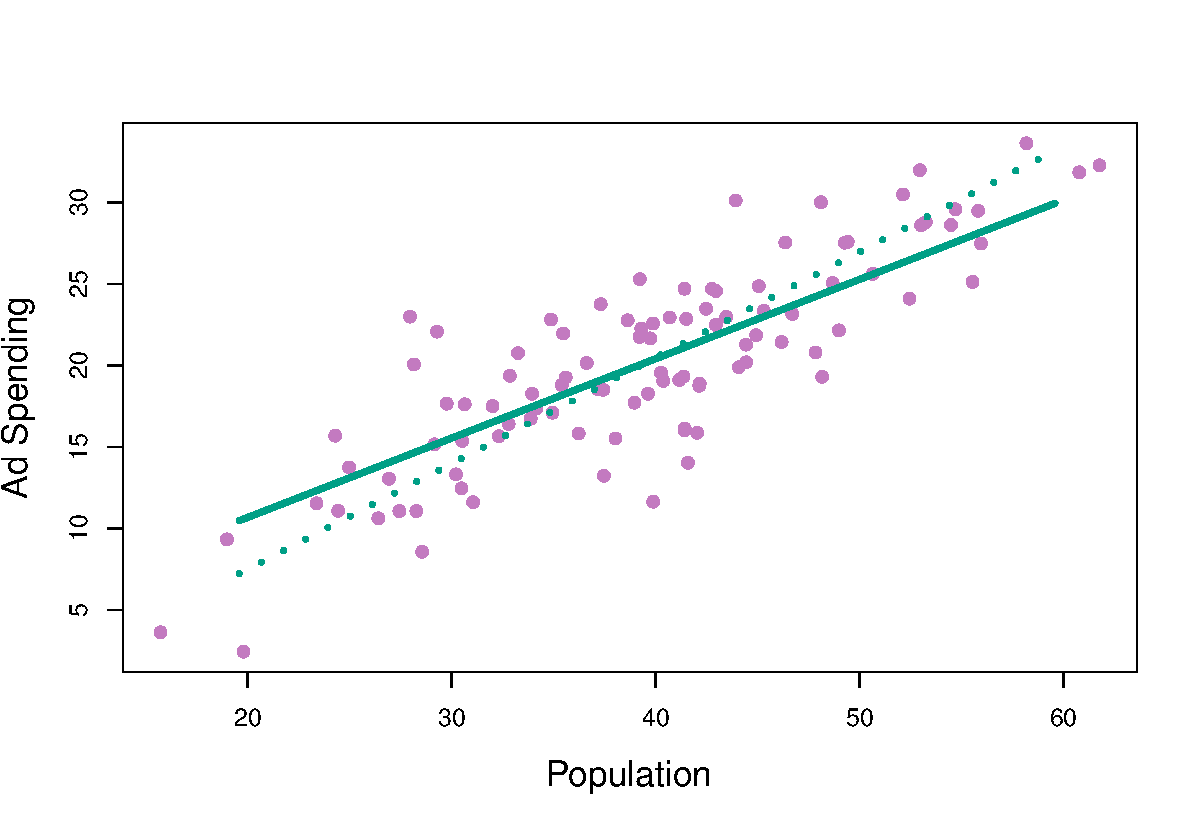
\includegraphics[scale=0.50]{IMG/PCAExample5.pdf}
\end{figure}
\vspace{-0.6cm}
\centering Sample dataset with 2 variables. The first PLS direction (component) -- solid line -- is shown. Compare to the PCA/PCR first direction (component) -- dotted line (shown previously).
\end{frame}
%---------------------------------------------------------------------
\begin{frame}{Partial least squares (PLS)}
Second component for PLS:\\
\medskip
\begin{enumerate}
    \item We regress each variable on $\bm{z}_1^{\textnormal{PLS}}$ and take residuals \\($\bm{x}_1 \leftarrow \bm{z}_1^{\textnormal{PLS}}$ and save OLS residuals $\ddot{\bm{x}}_1$; repeat for $\bm{x}_2$, etc.)\\~\\
    Individual $\ddot{\bm{x}}_j$ residuals can be interpreted as the ``remaining'' information of $\bm{x}_j$ that is not explained by the first PLS direction (component).\\
    \medskip
    \item Compute $\bm{z}_2^{\textnormal{PLS}}$ using the orthogonalized data ($\ddot{\bm{X}}$), \\the same way as the first component.\\
    (Run all $\bm{y} \leftarrow \ddot{\bm{x}}_j$ regressions and standardize coefficients).
\end{enumerate}
\bigskip
By analogy, this procedure can be repeated for all subsequent components.
\end{frame}
%---------------------------------------------------------------------
\begin{frame}{Partial least squares (PLS)}

The supervised dimension reduction in PLS can reduce bias \\(compared to PCR). \\~\\However, it can also increase variance of predictions. Hence, the benefits of using PLS over PCR can be outweighted by drawbacks ($k$FCV may be used to compare the two methods).\\~\\

PCR/PLS -- detailed technical description and estimation algorithm:
\begin{itemize}
\item (\textcolor{blue}{\underline{\href{https://cran.r-project.org/web/packages/pls/vignettes/pls-manual.pdf}{\{pls\} package manual}}})
\item (\textcolor{blue}{\underline{\href{https://web.stanford.edu/~hastie/ElemStatLearn/}{The Elements of 
Statistical Learning, ch. 3.5.1---3.5.2}}})
\end{itemize}
\end{frame}
%---------------------------------------------------------------------
\section{Moving beyond linearity}
\begin{frame}{Moving beyond linearity}
\end{frame}
%------------------------------------------------
\begin{frame}{Moving beyond linearity}
Different approaches are discussed (from simple to more complex), QREG is included mostly for reference.\\
\bigskip

\begin{itemize}
\item Quantile regression (quick repetition)
\smallskip
\item Polynomial and step (piecewise-constant) regression
\smallskip
\item Regression splines
\smallskip
\item Smoothing splines
\smallskip
\item Generalized Additive Models (GAM)
\end{itemize}
\end{frame}
%-------------------------------------------------------------------
\subsection{QREG - quick repetition}
\begin{frame}{QREG - quick repetition}
\begin{itemize}
\item Quantile regression estimates the relationship between regressors and a specified quantile of dependent variable.
\medskip
\item One important special case of quantile regression is the least absolute deviations (LAD) estimator, which corresponds to fitting the conditional median of the response variable ($q=\frac{1}{2}$).
\medskip
\item QREG (LAD) estimator can be motivated as a robust  alternative to OLS (with respect to outliers).
\medskip
\item Linear programming can be used for finding QREG estimates (Koenkerr and Bassett (around 1980).
\medskip
\item QREG-based predictions: Conditional quantiles (expected values) can be produced.
\medskip
\item To optimize prediction properties, QREG may be combined with parameter-shrinkage methods (lasso, ridge).
\end{itemize}
\end{frame}
%------------------------------------------------
\begin{frame}{Quantile regression (QREG)}
For LRMs, the $q$-th quantile regression estimator $\bm{\beta}_q$ minimizes:
$$
\underset{\bm{\hat{\beta}}_q}{\textnormal{min:}} \quad Q_n(\bm{\hat{\beta}}_q) =
\! \! \sum^n_{i:\, e_i \, \geq \, 0} q|y_i - \bm{x}_i\bm{\hat{\beta}}_q| \,\, +
\! \! \sum^n_{i:\, e_i\, < \, 0} (1-q)|y_i - \bm{x}_i\bm{\hat{\beta}}_q|,
$$
where $e_i = (y_i - \bm{x}_i\bm{\hat{\beta}}_q)$.

\begin{itemize}
    \item We use the notation $\bm{\hat{\beta}}_q$ to make clear that different choices of $q$ lead to different  $\bm{\hat{\beta}}$.
    \item Slope of the loss function $Q_n$ is asymmetrical \\(around $e_i=0$).
    \item The loss function is not differentiable (at $e_i=0$) \\$\rightarrow$ gradient methods are not applicable \\(linear programming can be used).
\end{itemize}
\end{frame}
%---------------------------------------------
\begin{frame}{Quantile regression example}
Example 7.10 (Greene): Income Elasticity of Credit Cards Expenditure\\
\medskip
\texttt{CCexpend} $\leftarrow$ \texttt{log(INCOME) + AGE + \#DEPENDANTS}
\centering
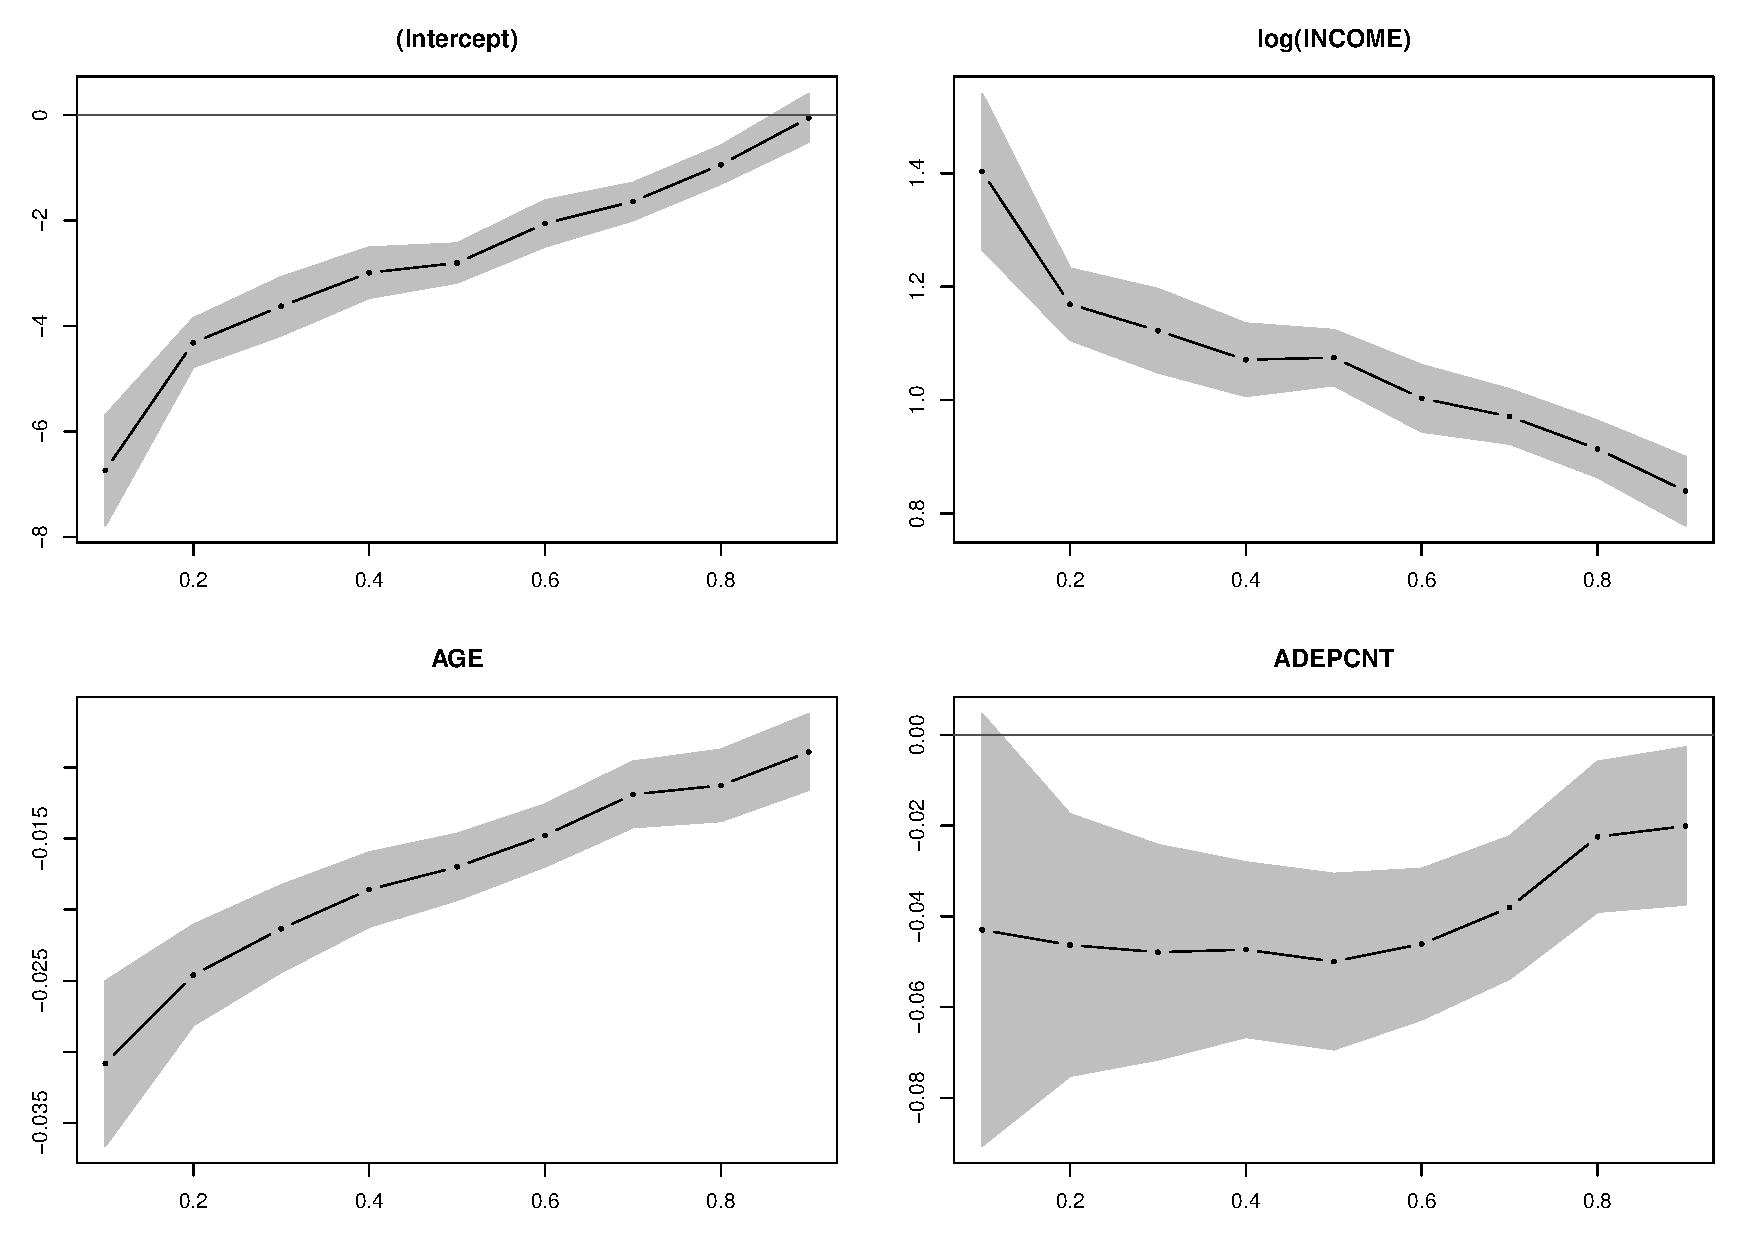
\includegraphics[width=10cm, height=6.7cm]{IMG/QREG.pdf}
\end{frame}
%---------------------------------------------
\subsection{Polynomial and step regression}
\begin{frame}{Polynomial regression}
Standard way to apply LRMs in situations where the relationship between a regressor and a dependent variable is non-linear.\\ \smallskip
\begin{itemize}
    \item Simple linear regression model $$y_i = \beta_0 + \beta_1 x_i + u_i,$$
    \item is replaced by a polynomial function (linear in parameters): 
    $$ y_i = \beta_0 + \beta_1 x_i + \beta_2 x_i^2 + \beta_3 x_i^3 + \dots  + \beta_d x_i^d + u_i .$$
    \item This approach extends easily to logistic regression models if $y_i$ is binary (applies to count and similar LDVs by analogy):
    $$\textnormal{Pr}(y_i=1|x_i) 
    = \frac{\exp(\beta_0 + \beta_1 x_i + \beta_2 x_i^2 + \beta_3 x_i^3 + \dots  + \beta_d x_i^d)}{1 + \exp(\beta_0 + \beta_1 x_i + \beta_2 x_i^2 + \beta_3 x_i^3 + \dots  + \beta_d x_i^d)} $$
    
\end{itemize}
\end{frame}
%---------------------------------------------
\begin{frame}{Polynomial regression (LRM \& logit examples)}
\centering
\medskip
\texttt{~~~~~~Wage} $\leftarrow$ \texttt{Age~~~~~~} \qquad \qquad \texttt{1[Wage>250]} $\leftarrow$ \texttt{Age}\\

\begin{figure}
  \centering
  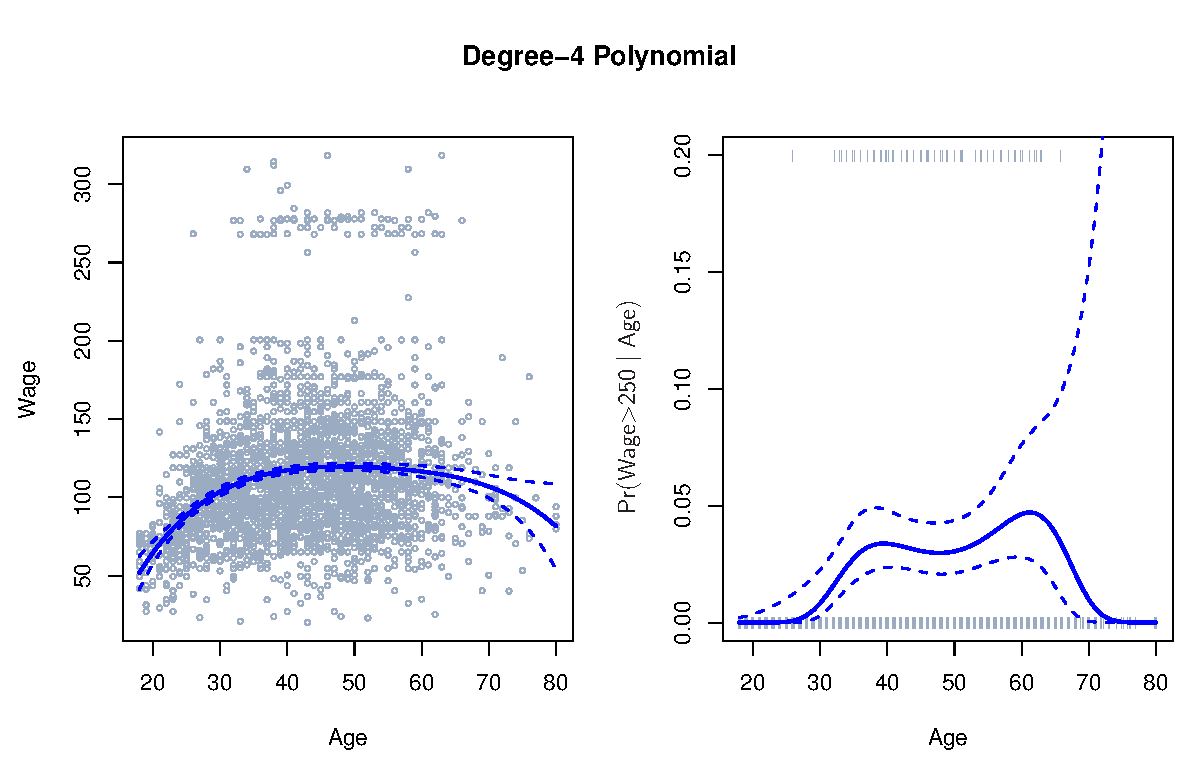
\includegraphics[trim=0cm 0cm 0cm 0cm, clip=true, width=0.9\textwidth]{IMG/ISLR71.pdf}
\end{figure}
\end{frame}
%---------------------------------------------
\begin{frame}{Polynomial regression}
\begin{itemize}
    \item Mostly, we are not interested in exact values of coeffcients.\\
    Usually, we seek to obtain ``good'' fitted values for some $x_0$: \\ \smallskip 
    $\hat{f}(x_0) = \hat{\beta}_0 + \hat{\beta}_1 x_0 + \hat{\beta}_2 x_0^2 + \dots + \hat{\beta}_d x_0^d $\\ \smallskip 
    and we study the general  prediction properties (variance, bias) \\of  $\hat{f}(x_0)$.
    \smallskip
    \item Either fix the $d$ at some low value (4 at most), or use cross-validation to choose $d$.
    \smallskip
    \item Caveat: polynomials have notorious tail behavior -- bad for extrapolation.
    \smallskip 
    \item We can use polynomials for several separate regressors in a LRM: we just stack the variables into one $\bm{X}$ matrix (see GAMs next).
    
\end{itemize}
\end{frame}
%---------------------------------------------
\begin{frame}{Step (piecewise-constant) regression}
\begin{itemize}
    \item Polynomial regression function imposes a \textit{global} structure on the non-linear function.
    \smallskip
    \item Instead, we can use a step function where regressor $x$ is broken into different bins and we fit a different constant for each bin (our regressor is transformed into a ordered categorical variable).
    \smallskip
    \item Alternatively, we select adequate (ad-hoc) cutpoints $c_1, c_2, \dots, c_K$ for a continuous regressor $x$ and construct $K+1$ dummy variables:
    \begin{equation*}
       \begin{aligned}
       C_0(X) \quad &= \quad 1[X < c_1], \\
       C_1(X) \quad &= \quad 1[c_1 \leq X < c_2], \\
        &~ \vdots \\
       C_{K-1}(X) \quad &= \quad 1[c_{K-1} \leq X < c_{K}], \\
       C_K(X) \quad &= \quad 1[c_{K} \leq X] \\
        \end{aligned}    
        \end{equation*}
\end{itemize}
\end{frame}
%---------------------------------------------
\begin{frame}{Step (piecewise-constant) regression}
\begin{itemize}
    \item Next, we use $C_0(X), C_1(X), C_2(X), \dots, C_K(X)$ to fit LRM:
    $$y_i = \beta_0 + \beta_1 C_1(x_i) + \beta_2 C_2(x_i) + \dots + \beta_K C_K(x_i) + u_i .$$
    $C_0$ is excluded from the model to avoid perfect multicolinearity. Exclusion is arbitrary -- any of the dummies may be excluded. Alternatively, we may include all dummies and drop $\beta_0$.
    \bigskip
    \item Again, this approach extends easily to logistic regression models if $y_i$ is binary (applies to count and similar LDVs by analogy):
    \small
    $$\textnormal{Pr}(y_i=1|x_i) 
    = \frac{\exp[\beta_0 + \beta_1 C_1(x_i) + \beta_2 C_2(x_i) + \dots + \beta_K C_K(x_i)]}{1 + \exp[\beta_0 + \beta_1 C_1(x_i) + \beta_2 C_2(x_i) + \dots + \beta_K C_K(x_i)]}. $$
\end{itemize}
\end{frame}
%---------------------------------------------
\begin{frame}{Piecewise-constant regression (LRM \& logit examples)}
\centering
\medskip
\texttt{~~~~~~Wage} $\leftarrow$ \texttt{Age~~~~~~} \qquad \qquad \texttt{1[Wage>250]} $\leftarrow$ \texttt{Age}\\
\begin{figure}
  \centering
  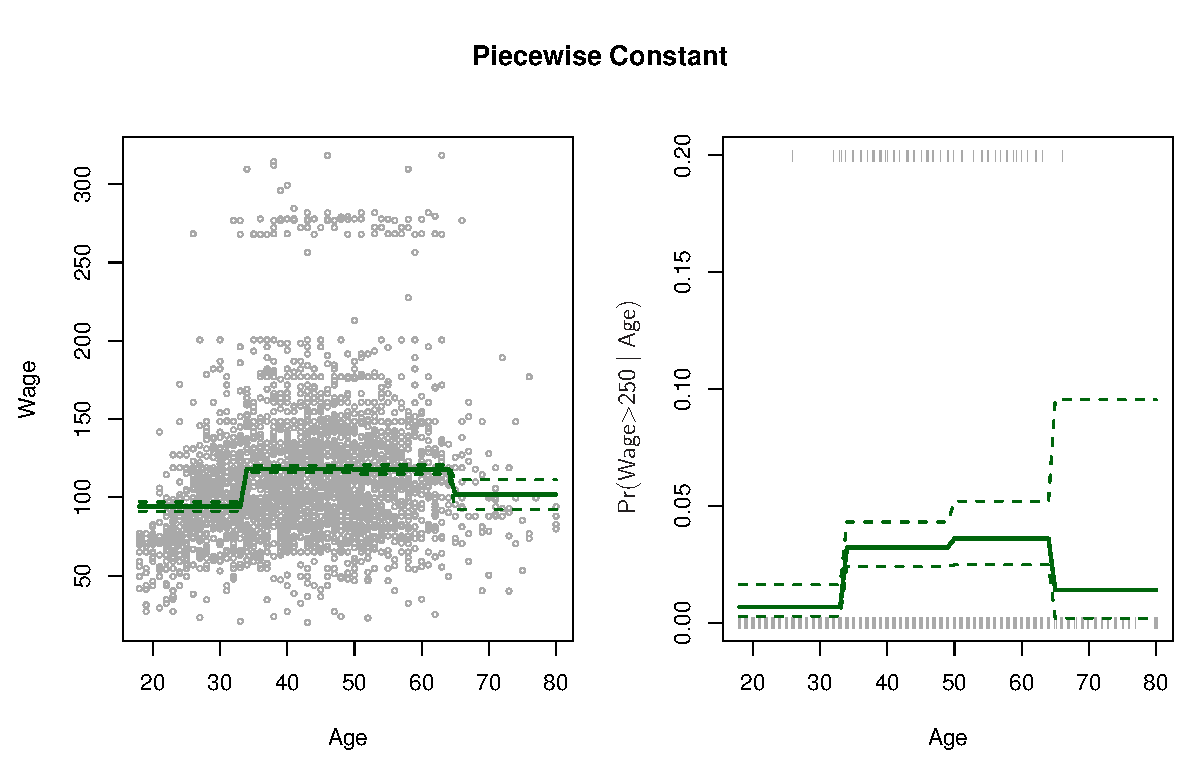
\includegraphics[trim=0cm 0cm 0cm 0cm, clip=true, width=0.9\textwidth]{IMG/ISLR72.pdf}
\end{figure}
\end{frame}
%---------------------------------------------
\begin{frame}{Step (piecewise-polynomial) regression}
Combines polynomial regression with step (piecewise) regression.

\bigskip
\textbf{Piecewise-polynomial regression:} \\Fit separate (low-degree) polynomials over different regions of $X$ \\(instead of one high-degree polynomial over the entire range of $X$). \\ \bigskip
Example: piecewise cubic polynomial with a single knot (cutpoint) $c_1$:
\medskip
\begin{equation*}
y_i = 
    \begin{cases}
        \beta_{01} + \beta_{11} x_i + \beta_{21} x_i^2 + \beta_{31} x_i^3 + u_i \textnormal{~~if~~} x_i <  c_1 ;& \\ ~ & \\
         \beta_{02} + \beta_{12} x_i + \beta_{22} x_i^2 + \beta_{32} x_i^3 + u_i \textnormal{~~if~~} x_i \geq  c_1 .& 
    \end{cases}
\end{equation*}
\medskip
\begin{itemize}
    \item Here, we fit two different polynomials to the data.
    \item For $K$ knots (cutpoints), we fit $K+1$ different polynomials.\\(i.e. with one knot, twice as much parameters are estimated) 
    \item Different $d$ are possible: $d=1~\rightarrow~$ piecewise linear function.
\end{itemize}
\end{frame}
%---------------------------------------------
\begin{frame}{Step (piecewise-polynomial) regression}
Example: piecewise cubic polynomial with one knot:\\
\centering
\medskip
\texttt{Wage} $\leftarrow$ \texttt{Age}\\
\vspace{-0.2cm}
\begin{figure}
  \centering
  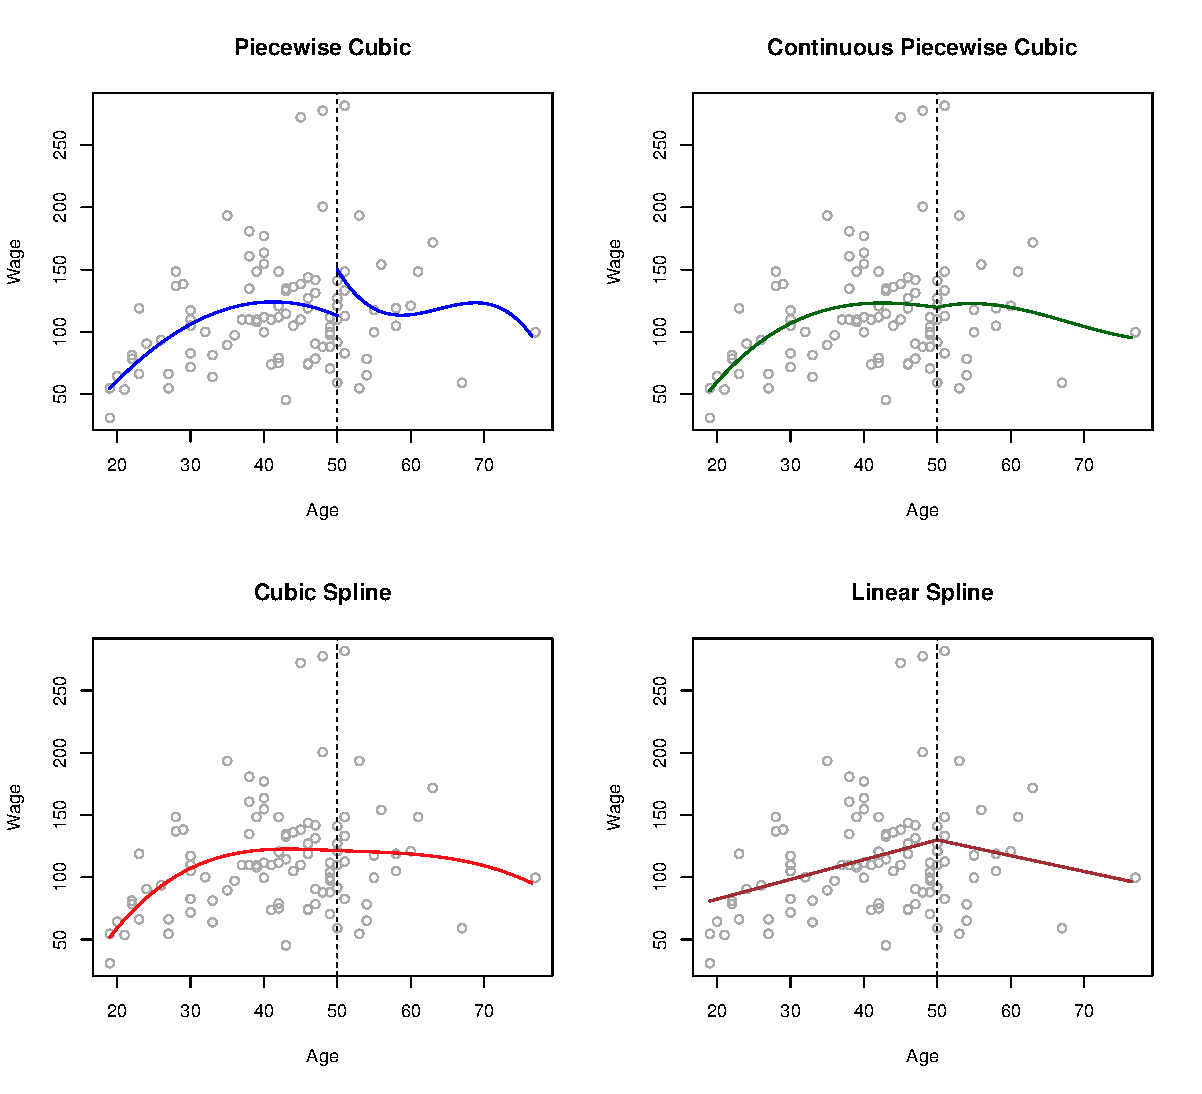
\includegraphics[trim=0cm 9.5cm 10.5cm 0cm, clip=true, width=0.4\textwidth]{IMG/ISLR73.pdf}
\end{figure}

\vspace{-0.5cm}
\begin{itemize}
    \item[\ding{51}] Improved flexibility
    \item[\ding{55}] Fitted curve non-continuous
\end{itemize}
\end{frame}
%---------------------------------------------
\subsection{Regression splines and smoothing splines}
\begin{frame}{Regression splines - motivation}
\centering
Piecewise linear regression with one knot at $c_1$:\\
\vspace{-0.2cm}
\begin{figure}
  \centering
  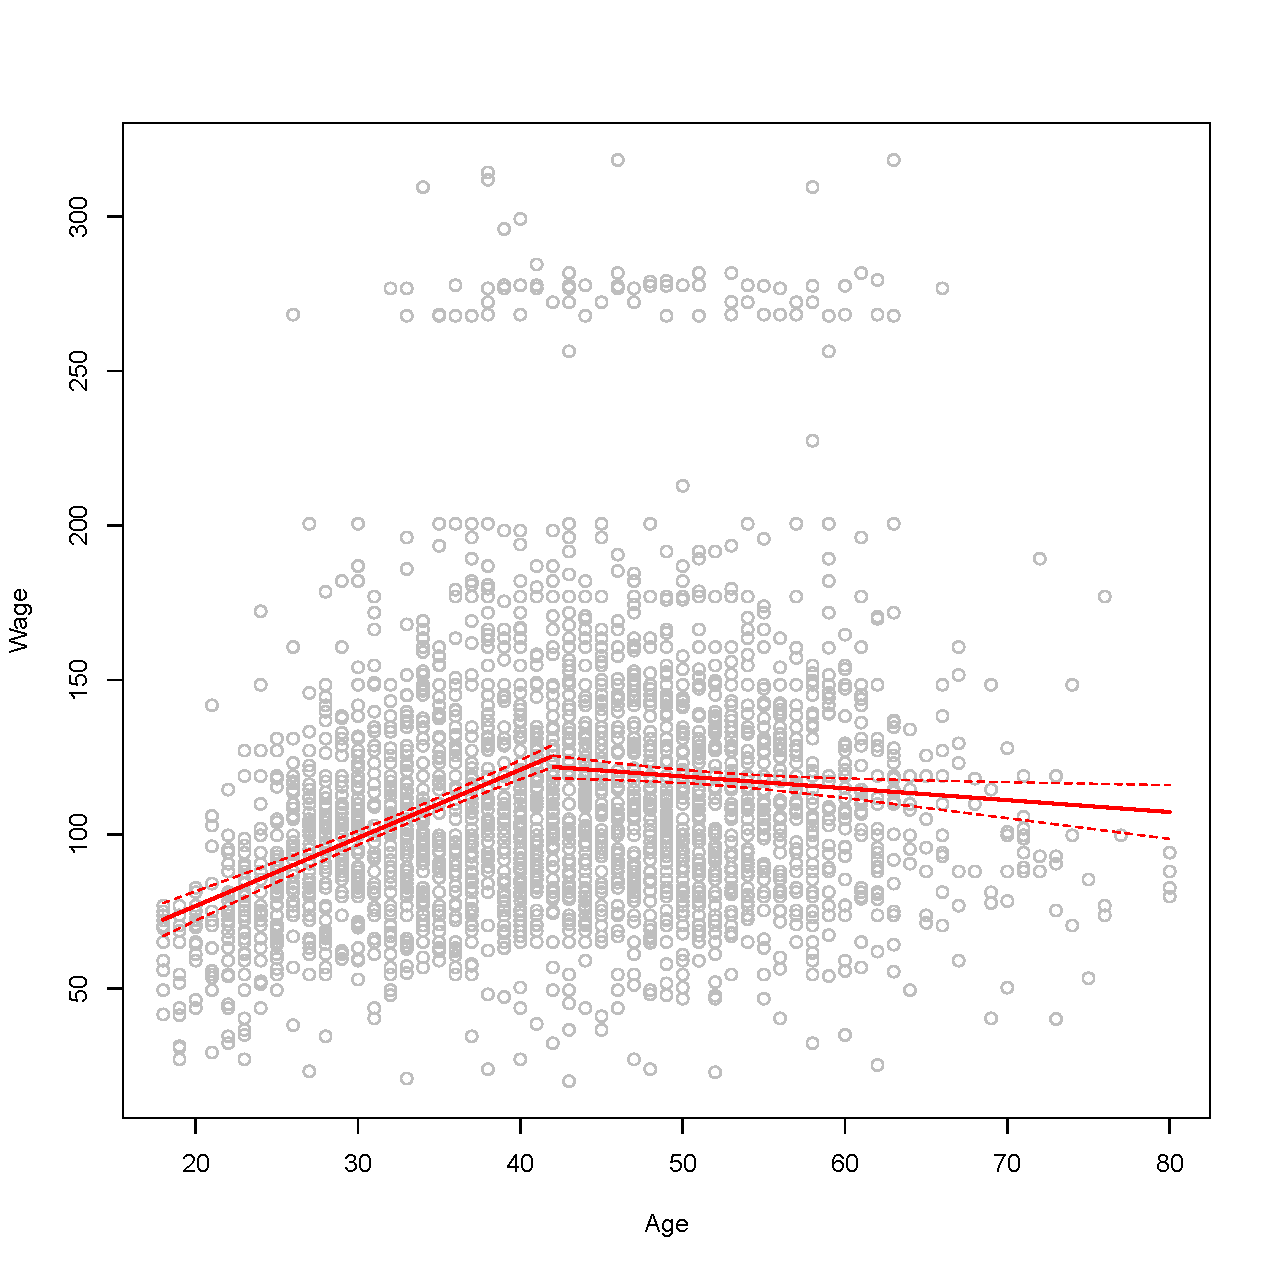
\includegraphics[trim=0cm 0cm 0cm 0cm, clip=true, width=0.4\textwidth]{IMG/ISLR73a.pdf}
\end{figure}
\vspace{-0.2cm}
\begin{equation*}
y_i = 
    \begin{cases}
        \beta_{01} + \beta_{11} x_i + u_i \textnormal{~~if~~} x_i <  c_1 ;& \\ ~ & \\
         \beta_{02} + \beta_{12} x_i + u_i \textnormal{~~if~~} x_i \geq  c_1 .& 
    \end{cases}
\end{equation*}
\end{frame}
%---------------------------------------------
\begin{frame}{Regression splines}
\centering
Piecewise linear ``continuous'' regression with one knot at $c_1$:\\
\vspace{-0.2cm}
\begin{figure}
  \centering
  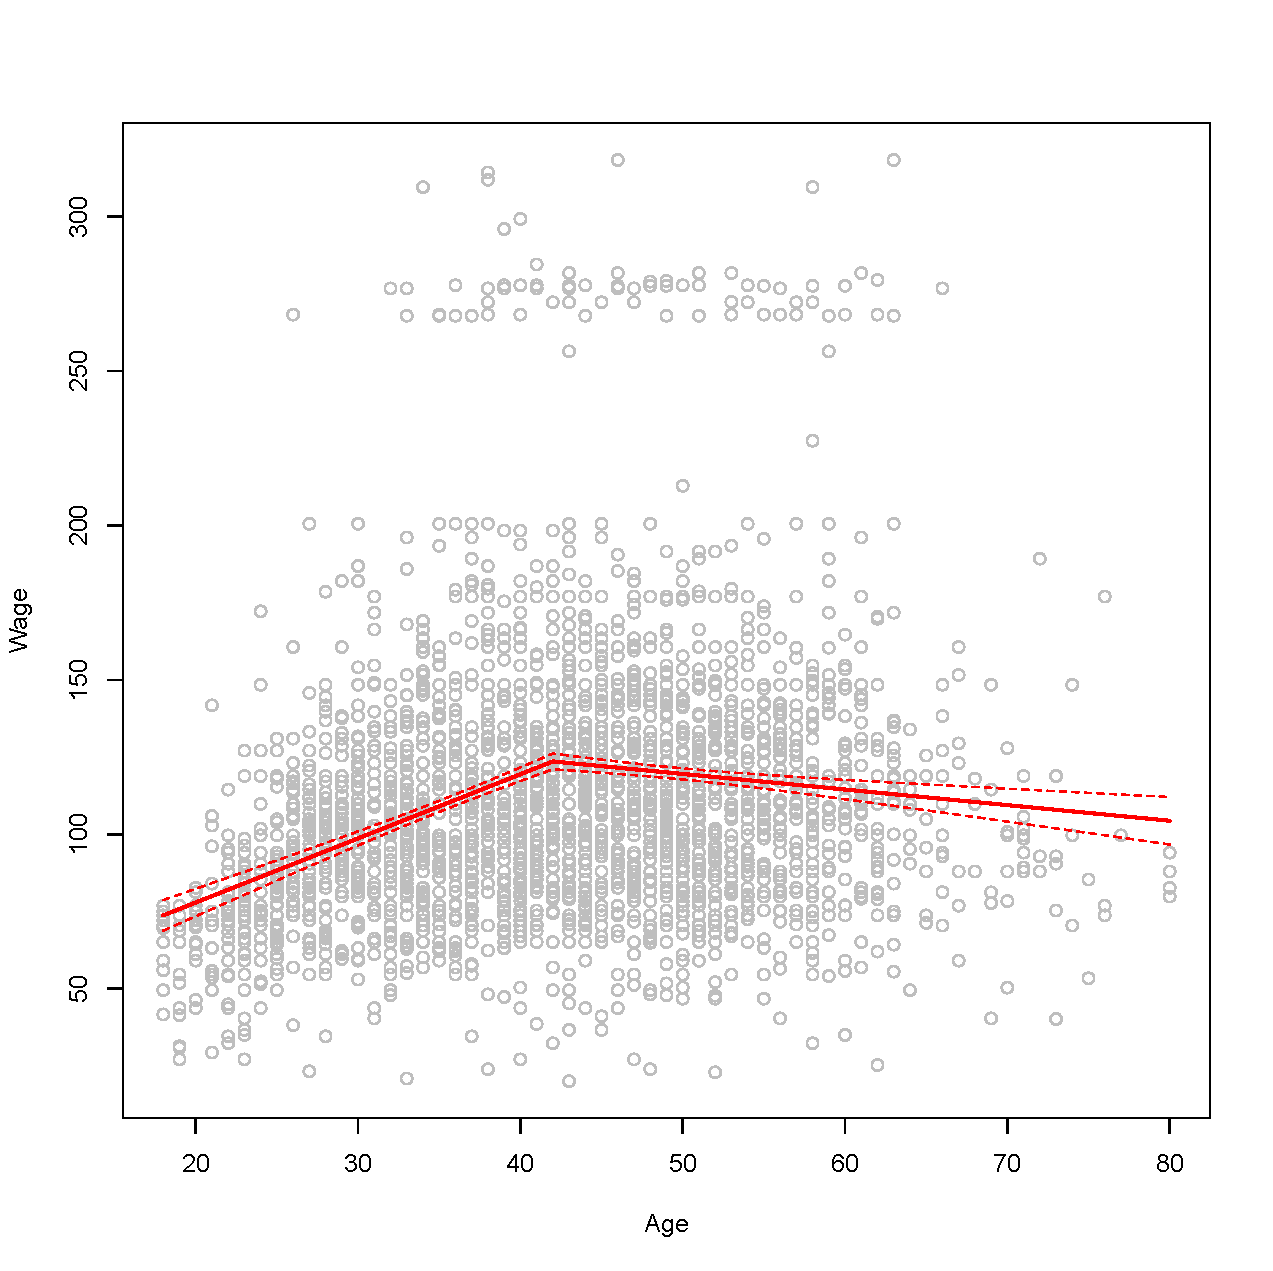
\includegraphics[trim=0cm 0cm 0cm 0cm, clip=true, width=0.4\textwidth]{IMG/ISLR73b.pdf}
\end{figure}
\vspace{-0.5cm}
``Continuity'' can be easily imposed as follows:
$$ y_i = \beta_0 + \beta_1x_i + \beta_2\{1[x_i > c_1](x_i-c_1)\} + u_i$$
\end{frame}
%---------------------------------------------
\begin{frame}{Regression splines (linear spline)}
\textbf{Linear spline:} fit regression line in each region of the predictor space, requiring continuity in each knot. Regression model with $K$ knots $\xi_k, k=1,\dots, K$ can be represented using \textcolor{blue}{basis functions} as follows:
$$y_i = \beta_0 + \beta_1 \, b_1 (x_i) + \beta_2 \, b_2 (x_i) + \cdots  + \beta_{K+1} \, b_{K+1} (x_i) + u_i  $$
where $b_k$ are the basis functions:\\
\smallskip
\qquad $b_1 (x_i) = x_i$\,,\\
\qquad $b_2 (x_i) = (x_i-\xi_1)_{+} = 1[x_i > \xi_1](x_i-\xi_1)\}$,\\
\qquad $b_3 (x_i) = (x_i-\xi_2)_{+}$\,, \\ \qquad etc.\\
\medskip
\begin{itemize}
    \item The $(x_i-\xi_k)_{+}$ means the positive part of the difference.
    \smallskip
    \item With linear splines, each knot only adds one estimated parameter to the estimation, i.e. $K\!+\!2\,$ d.f. are used (compare to non-continuous piecewise linear regression: $2K$ d.f. used).
    \smallskip
    \item Basis functions (notation) will be useful in subsequent discussion.
\end{itemize}
\end{frame}
%---------------------------------------------
\begin{frame}{Regression splines (cubic spline)}
\textbf{Cubic spline} with knots $\xi_k,~k=1,\dots, K$ is a piecewise cubic polynomial with continuous derivatives up to order 2 at each knot.\\
\medskip
Again we can represent this model with truncated power basis functions:
$$y_i = \beta_0 + \beta_1 \, h_1 (x_i) + \beta_2 \, h_2 (x_i) + \cdots + \beta_{K+3} \, h_{K+3} (x_i) + u_i  $$
where:\\
\smallskip
\qquad $h_1 (x_i) = x_i$\,,\\
\smallskip
\qquad $h_2 (x_i) = x_i^2$\,,\\
\smallskip
\qquad $h_3 (x_i) = x_i^3$\,,\\
\smallskip
\qquad $h_4 (x_i) = (x_i-\xi_1)_{+}^3 \,$ \qquad (note that $h_4 = h_{k+3}$)\,,\\
\smallskip
\qquad $h_5 (x_i) = (x_i-\xi_2)_{+}^3 \,$ ,\\
\qquad $\cdots$ \\
\qquad $h_{K+3} (x_i) = (x_i-\xi_K)_{+}^3 \,$.\\
\medskip
\end{frame}
%---------------------------------------------
\begin{frame}{Regression splines (cubic spline)}
\centering
\vspace{-0.2cm}
\begin{figure}
  \centering
  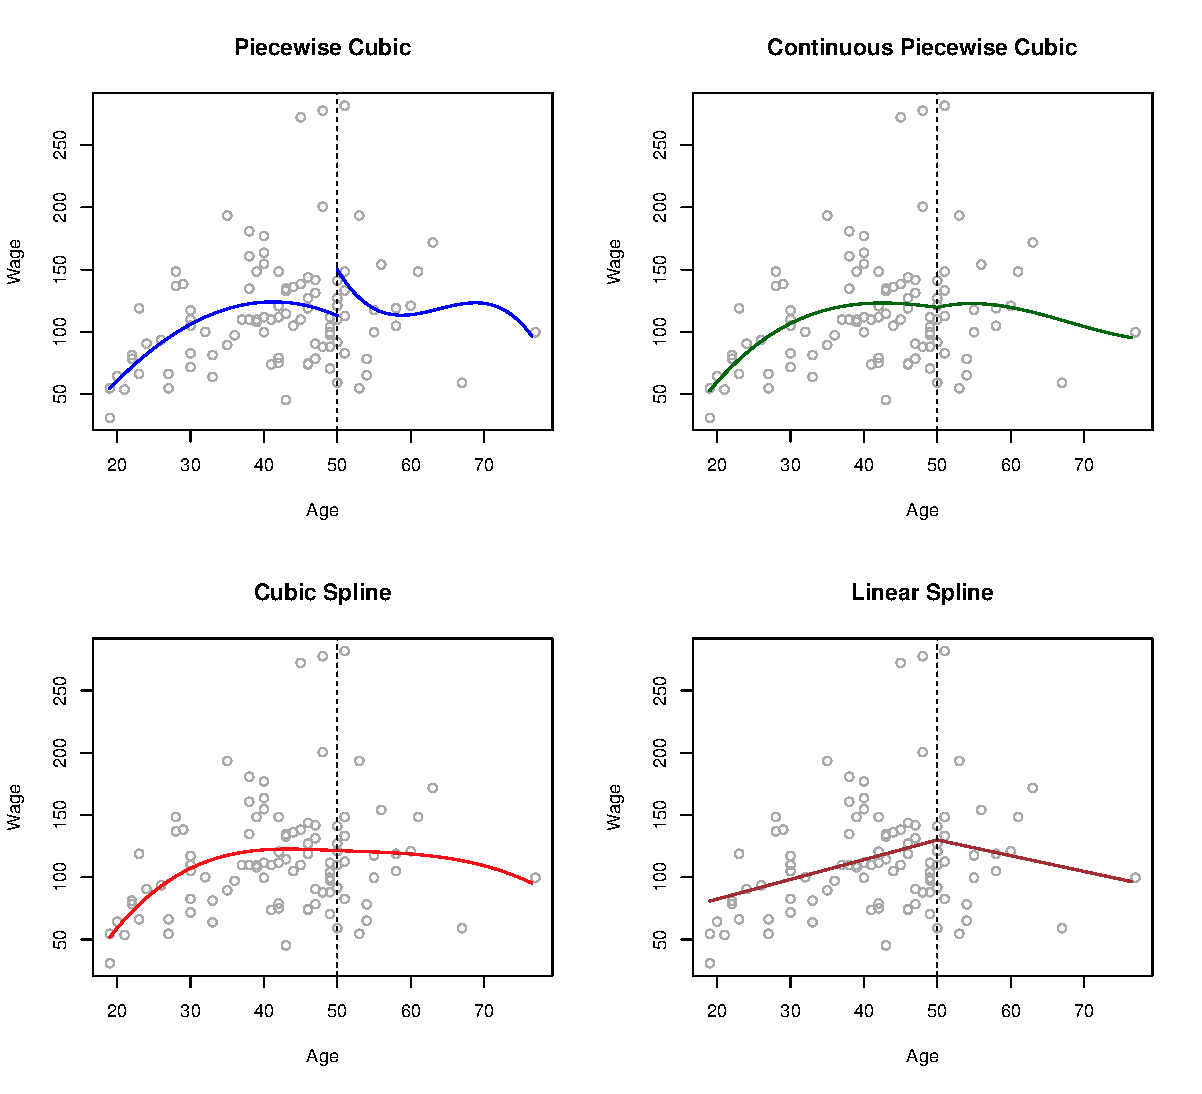
\includegraphics[trim=0cm 0cm 0cm 0cm, clip=true, width=0.75\textwidth]{IMG/ISLR73.pdf}
\end{figure}
\end{frame}
%---------------------------------------------
\begin{frame}{Regression splines (cubic spline)}
\begin{itemize}
    \item Cubic spline uses $4+K$ d.f.
    \smallskip
    \item Cubic spline has continuous derivatives up to order 2 at each knot.\\
    $d$-spline (degree-$d$ spline) has continuous derivatives up to degree $d-1$ at each knot.
    \smallskip
    \item Cubic spline popularity is based on human perception: this is the lowest-order spline where knot-discontinuity is not visible to the human eye.
    \smallskip
    \item Unfortunately, $d$-splines (incl. cubic splines) tend to have high variance at the outer range of the predictor (i.e. when $X$ is very low or very high). Possible solution: use ``natural splines'' with additional boundary constraints.
\end{itemize}
\end{frame}
%---------------------------------------------
\begin{frame}{Regression splines (natural spline)}
\textbf{Natural cubic spline:} a cubic regression spline with additional boundary constraints:\\
\smallskip
\begin{itemize}
    \item For a cubic spline regression model $y \leftarrow x$ with $K$ knots, \\$f(X)$ is required to be linear for $X \leq \xi_1$ and for $X > \xi_K$.
    \smallskip
    \item Additional restrictions free 4 d.f. (compared to cubic spline), \\so we use $K$ d.f. for estimation.
\end{itemize}
\vspace{-0.4cm}
\begin{figure}
  \centering
  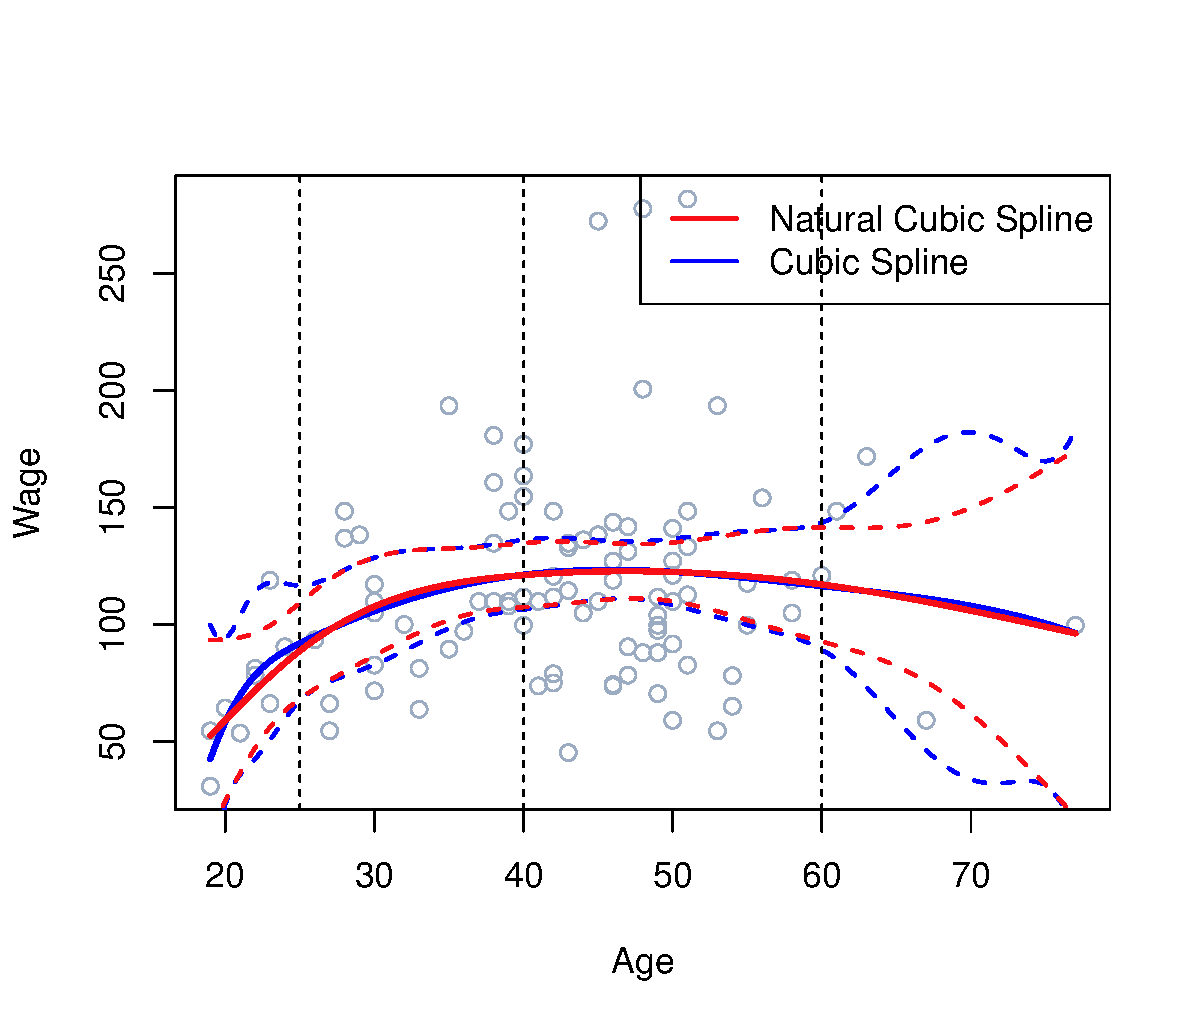
\includegraphics[trim=0cm 0cm 0cm 1cm, clip=true, width=0.5\textwidth]{IMG/ISLR74.pdf}
\end{figure}
\end{frame}
%---------------------------------------------
\begin{frame}{Regression splines (natural spline)}
Example: For $K\!=\!4$ and using the truncated power bases of cubic splines $(X-\xi_k)_{+}^3 \,$, we can write:
$$y_i = \beta_0 \, N_1 (x_i)  + \beta_1 \, N_2 (x_i) + \beta_2 \, N_3 (x_i) + \beta_3 \, N_4 (x_i) + u_i  $$\\
\vspace{-0.2cm}
where:\\
\smallskip
\qquad $N_1 (x_i) = 1$\, \hspace{3.5cm} ~($\beta_0$ is the intercept),\\
\smallskip
\qquad $N_2 (x_i) = x_i$\,,\\
\smallskip
\qquad $N_3 (x_i) = d_1(X)-d_{3}(X)$ \qquad \qquad (note that $N_3=N_{k+2}$),\\
\smallskip
\qquad $N_4 (x_i) = d_2(X)-d_{3}(X)$\\
\medskip
\qquad and $d_k(X)=\frac{(X-\xi_k)_{+}^3 \,-\, (X-\xi_K)_{+}^3}{\xi_K \,-\, \xi_k}$.\\
\bigskip
For basis functions, we only use knots up to $K\!-\!2$ (i.e. $\xi_1, \xi_2$ for $K\!=\!4$).
\end{frame}
%---------------------------------------------
\begin{frame}{Regression splines (natural spline)}
General notation for natural cubic splines with $K$ knots:
$$y_i = \beta_0 \, N_1 (x_i)  + \beta_1 \, N_2 (x_i) + \beta_2 \, N_{k+2} (x_i) + \cdots + \beta_{K-3} \, N_{K-2} (x_i) + u_i  $$\\
\vspace{-0.2cm}
~\,where:\\
\smallskip
\qquad $N_1 (x_i) = 1$\,,\\
\smallskip
\qquad $N_2 (x_i) = x_i$\,,\\
\smallskip
\qquad $N_{k+2} (x_i) = d_k(X)-d_{K-1}(X)\,$,\\
\qquad $\cdots$\\
\qquad $N_{K-2} (x_i) = d_{K-2}(X)-d_{K-1}(X)\,$,\\
\bigskip
\qquad and $d_k(X)=\frac{(X-\xi_k)_{+}^3 - \, (X-\xi_K)_{+}^3}{\xi_K \,-\, \xi_k}$.\\
\bigskip
All basis functions $N_1,N_2,N_{k+2},\dots,N_{K-2}$ have $2^{nd}$ and $3^{rd}$ derivatives \\equal to zero for $X < \xi_1$ and for $X \geq \xi_K$.
\end{frame}
%---------------------------------------------
\begin{frame}{Regression splines (knot selection)}
Where should we place the knots?\\
\bigskip
\begin{itemize}
    \item Specify the number of knots and use uniformly distributed quantiles.\\
    \medskip    
    \begin{itemize}
        \item 1 knot: at median, 2 knots: at $q_{0.33}$ and $q_{0.66\,}$, etc.
        \smallskip
        \item Optimum number of knots can be determined by $k$FCV.
    \end{itemize}
    \bigskip
    \item Spline function is most flexible in regions that contain a lot of knots. Hence:\\
    \medskip    
    \begin{itemize}
        \item Place more knots in regions where we assume the function \\may vary most rapidly.
        \smallskip
        \item Place fewer knots where the function seems more stable.
        \smallskip
        \item Ad-hoc and potentially misleading approach.
    \end{itemize}
\end{itemize}
\end{frame}
%---------------------------------------------
\begin{frame}{Smoothing splines (quick overview)}
\begin{itemize}
    \item Smoothing splines -- alternative approach to splines.\\
    \bigskip
    \item Search for a function $g(x)$ that minimizes RSS and is smooth.
\end{itemize} \medskip
$$\min:~~~\textnormal{RSS}(g,\lambda) = \sum_{i=1}^n [y_i - g(x_i)]^2 + \lambda \int g''(t)^2 \textit{dt}$$
\begin{itemize}
    \item $\sum_{i=1}^n [y_i - g(x_i)]^2$ is a loss function, makes $g(x)$ fit the data.\\  \smallskip
    $g(x)$ can be any function for which the second term is defined.\\
    \bigskip
    \item $\lambda \int \! g''(t)^2 \textit{dt}~$ penalizes high variability in $g(x)$.\\  \smallskip
    $\lambda$ is a penalty term. For $\lambda=\infty$, smoothing splines lead to OLS fit.
\end{itemize}
\end{frame}
%---------------------------------------------
\begin{frame}{Smoothing splines (quick overview)}
$$\min:~~~\textnormal{RSS}(g,\lambda) = \sum_{i=1}^n [y_i - g(x_i)]^2 + \lambda \int g''(t)^2 \textit{dt}$$
\begin{itemize}
    \item $g'(t)$ is the first derivative, measures slope of $g(t)$ at $t$.\\
    \smallskip
    $g''(t)$ indicates $2^{nd}$ derivative and corresponds to the amount \\by which the slope is changing.
    \medskip
    \item $g''(t)$ is a measure of ``\textit{roughness}'' of $g(t)$ around $t$.\\
    \smallskip
    it is large (in absolute value) if $g(t)$ is ``wiggly'' near $t$,\\
    \smallskip
    it is zero if $g(t)$ is a straight line around $t$.
    \medskip
    \item $\int g''(t)^2 \textit{dt}$ ~is a (specific) measure of the total change in $g'(t)$ \\over the entire range. 
\end{itemize}
\end{frame}
%---------------------------------------------
\begin{frame}{Smoothing splines (quick overview)}
$$\min:~~~\textnormal{RSS}(g,\lambda) = \sum_{i=1}^n [y_i - g(x_i)]^2 + \lambda \int g''(t)^2 \textit{dt}$$
\begin{itemize}
    \item While $g$ can be any function, it may be shown that $\textnormal{RSS}(g,\lambda)$ has an explicit \& unique minimizer: natural cubic spline with $N$ knots at the unique values of $x_i,~i=1,2,\dots,N$. \\(more precisely, a penalized natural cubic spline with $N$ knots)
    \medskip
    \item With a suitable $\lambda$ parameter, the model is not overparameterized: \textcolor{blue}{effective degrees of freedom} used for estimation $(df_{\lambda})$ decrease from $N$ to 2 as $\lambda$ increases from 0 to $\infty$.
    \medskip
    \item Cross-validation can be used to find $\lambda$ with the lowest cross-validated RSS (LOOC is computationally very efficient here).
    \vspace{-0.3cm}
    \item For technical discussion of smoothing splines, see (\textcolor{blue}{\underline{\href{https://web.stanford.edu/~hastie/ElemStatLearn/}{ESL, ch. 5.4}}}).
\end{itemize}
\end{frame}
%---------------------------------------------
\begin{frame}{Smoothing splines (quick overview)}
\vspace{-0.4cm}
\begin{figure}
  \centering
  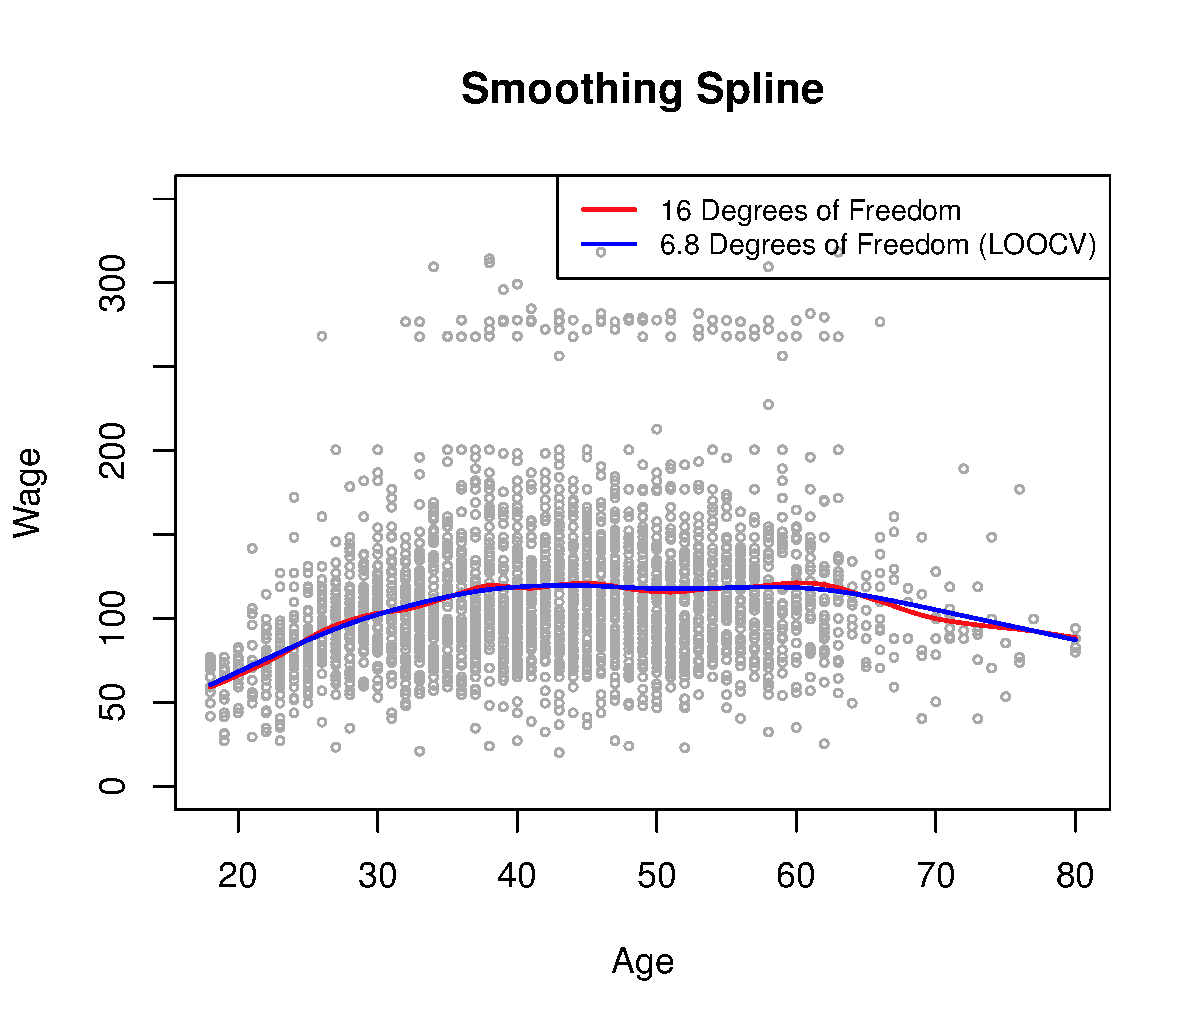
\includegraphics[trim=0cm 0cm 0cm 1cm, clip=true, width=0.6\textwidth]{IMG/ISLR78.pdf}
\end{figure}
\centering
\vspace{-0.5cm}
\tiny{Note that \textit{df} in the legend refer to $(df_{\lambda})$ used by the estimation.}
\end{frame}
%---------------------------------------------
\subsection{Local regression}
\begin{frame}{Local regression}
\begin{itemize}
    \item Another approach for fitting flexible (non-linear) functions.
    \item For a given target point $x_0$, regression is fit using nearby observations only.
\end{itemize}
\bigskip
\centering
Local regression example (artificial data)
\vspace{-0.4cm}
\begin{figure}
  \centering
  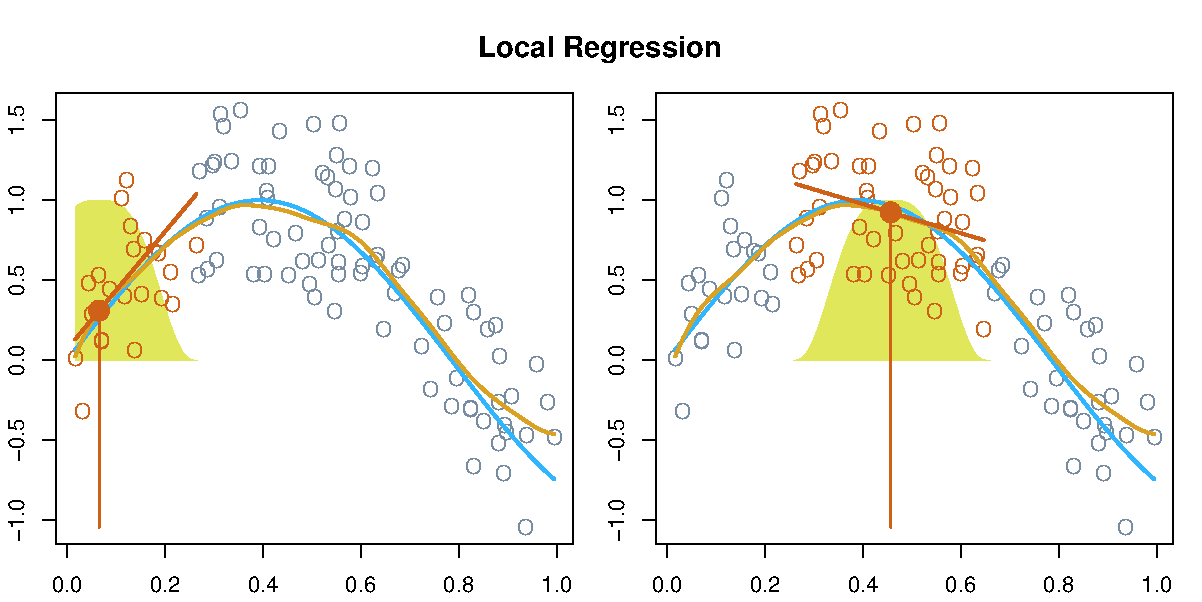
\includegraphics[trim=0cm 0cm 0cm 1.1cm, clip=true, width=0.7\textwidth]{IMG/ISLR79.pdf}
\end{figure}
\vspace{-0.4cm}
\tiny{Legend: orange: local regression, blue: DGP, yellow bell: weight of observations used in regression.}
\end{frame}
%---------------------------------------------
\begin{frame}{Local regression algorithm}
Local regression at $X = x_0$\\
\bigskip
\begin{enumerate}
    \item Gather the fraction $s = k/n$ of training points whose $x_i$ \\are closest to $x_0$.
    \medskip
    \item Assign a weight $K_{i0} = K(x_i , x_0)$ to each point in this neighborhood, so that the closest point has the highest weight \\and vice versa. All but the nearest $k$ neighbors get zero weights.
    \medskip
    \item Fit \textit{weighted least squares regression} of $y_i$ on $x_i$ by finding $\beta$ parameters that minimize the following expression:
    $$\min : ~~~ \sum_{i=1}^n K_{i0} (y_i - \beta_0 - \beta_1 x_i)^2 \,.$$
    \item Fitted value at $x_0$ is given by $\hat{f}(x_0) = \hat{\beta}_0 + \hat{\beta}_1 x_0\,$.
\end{enumerate}
\end{frame}
%---------------------------------------------
\begin{frame}{Local regression}
\textbf{Local regression: choices to be made}\\
\smallskip
\begin{itemize}
    \item Weighting function $K$ must be defined (e.g.: $\tfrac{1}{(x_0 - x_i)^2}, x_0 \neq x_i$).
    \smallskip
    \item Functional form in Step 3 (constant, linear, quadratic, etc.).
    \smallskip
    \item Span $s$ controls flexibility of the fit (can choose using CV).
\end{itemize}
\bigskip
\textbf{Local regression: notes}\\
\smallskip
\begin{itemize}
    \item Local regression can be generalized to models with multiple regressors: the model is global in some regressors and local in others (time). Such model adapts to the most recently gathered observations.
    \smallskip
    \item Local regression can be generalized to neighborhoods of higher dimensions (say, over $X_1$ and $X_2$). However, this approach does not extend easily to higher dimensions (beyond 3 or 4).
\end{itemize}
\end{frame}
%---------------------------------------------
\subsection{Generalized Additive Models (GAM)}
\begin{frame}{Generalized Additive Models (GAM)}
So far, polynomial and step regression, splines and local regression have been discussed as univariate regression models with $y_i \leftarrow f(x_i)$.\\
\medskip GAMs extend multivariate LRMs by allowing non-linear functions\\ \& smoothers in each variable, while maintaining additivity (and easy interpretation for each regressor).\\ \medskip
Multiple-regressor LRM:
$$ y_i = \beta_0 + \beta_1 x_{i1} + \beta_2 x_{i2} + \cdots + \beta_p x_{ip} + u_i~~~~~~~~~~~~~~~~~$$
can be generalized to a GAM:
$$ y_i = \alpha + \, f_1(x_{i1}) + \, f_2(x_{i2}) + \cdots + \, f_p(x_{ip}) + u_i$$ 
where each $f_j(x_{ij})$ represents any convenient function of $x$: piecewise constant, linear, polynomial, spline, etc.
\end{frame}
%---------------------------------------------
\begin{frame}{GAM example}
$$\texttt{wage} = \alpha + f_1(\texttt{year}) + f_2(\texttt{age}) + f_3(\texttt{education}) + u_i$$
\bigskip
where $f_1$ and $f_2$ are smoothing splines and $f_3$ is a step function (\texttt{education} is a qualitative variable with five levels).
\vspace{-0.2cm}
\begin{figure}
  \centering
  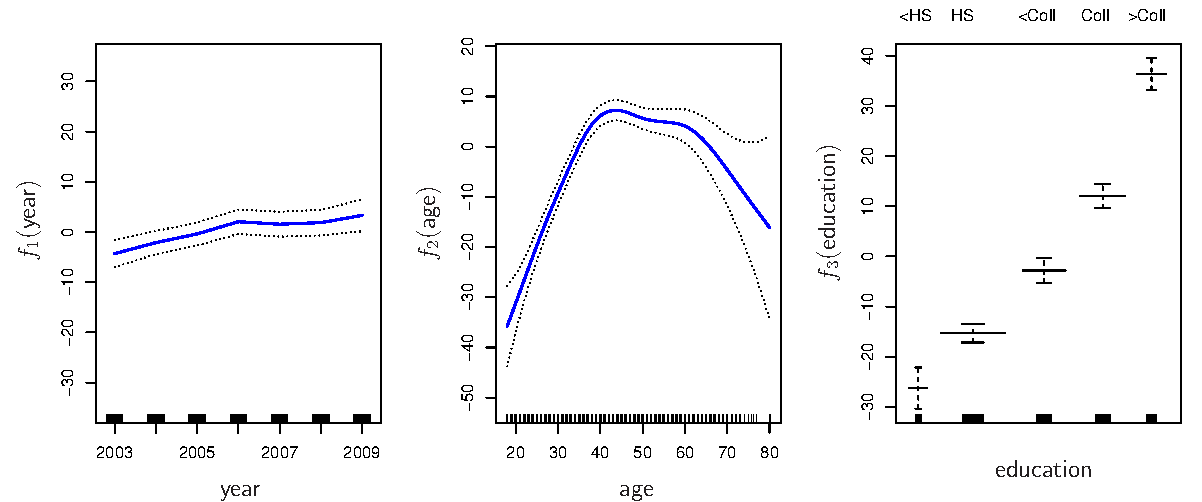
\includegraphics[trim=0cm 0cm 0cm 0cm, clip=true, width=0.85\textwidth]{IMG/ISLR712.pdf}
\end{figure}
\centering
\vspace{-0.3cm}
\tiny
As we hold \texttt{age} and \texttt{education} fixed, \texttt{wage} increases slightly with \texttt{year}.\\
If we fix \texttt{year} and \texttt{education}, than \texttt{wage} tends to be highest for intermediate \\values of  \texttt{age} and lowest for the very young and very old workers.
\end{frame}
%---------------------------------------------
\begin{frame}{GAM estimation (backfitting)}
\vspace{-0.3cm}
$$ y_i = \alpha + f_1(x_{i1}) + f_2(x_{i2}) + \cdots + f_p(x_{ip}) + u_i$$
\vspace{-0.3cm}
\begin{itemize}
    \item $f_j$ functions are unspecified smooth (``nonparametric'') functions.
    \smallskip
    \item With smoothing splines, we do not use an expansion of basis functions for estimation (i.e. constituent elements used in some matrix of regressors $\bm{X}$).
    \smallskip
    \item Instead, we fit all $p$ functions ``simultaneously'', using a scatterplot smoother (e.g. smoothing spline, local regression, etc.) along with a \textbf{backfitting algorithm}.
    \smallskip
    \item Say, we use cubic smoothing splines for all regressors. The penalized RSS (PRSS) can be specified as:
    \small{$$\textnormal{PRSS}(\alpha,f_1,\dots,f_p,\bm{\lambda}) = \sum_{i=1}^n \left[y_i - \alpha - \sum_{j=1}^p f_j(x_{ij}) \right]^2 + \sum_{j=1}^p \lambda_j \int f_j''(t_j)^2 \textit{dt}_j\,,$$}
    where $\lambda_j \geq 0$ and PRSS is used for estimaton (described next).
\end{itemize}
\end{frame}
%---------------------------------------------
\begin{frame}{GAM estimation (backfitting)}
\vspace{-0.3cm}
$$ y_i = \alpha + f_1(x_{i1}) + f_2(x_{i2}) + \cdots + f_p(x_{ip}) + u_i$$\\
\bigskip
\textbf{Backfitting algorithm for GAMs}\\ \medskip
\begin{enumerate}
    \item Initialize: $\hat{\alpha}=\frac{1}{n} \sum_{i=1}^n y_i~~\textnormal{and}~~\hat{f}_j \equiv 0,~~\forall i,j.$
    \bigskip
    \item Cycle: $j = 1,2,\dots,p,1,2,\dots,p,\dots$
    \bigskip
    \begin{itemize}
        \item[(a)] $\hat{f}_j~\leftarrow ~ \mathcal{S}_j \left[ \left\lbrace y_i - \hat{\alpha} - \sum_{k \neq j} \hat{f}_k (x_{ik}) \right\rbrace_1^n \right]~~~$(backfitting step)
        \bigskip
        \item[(b)] $\hat{f}_j~\leftarrow ~ \hat{f}_j - \frac{1}{n} \sum_{i-1}^n \hat{f}_j (x_{ij}) ~~~$(mean centering of estimated function)\\
        \bigskip
        until functions $\hat{f}_j$ change less than a prespecified threshold.
    \end{itemize}
\end{enumerate}
\end{frame}
%---------------------------------------------
\begin{frame}{GAM estimation (backfitting)}
\textbf{Backfitting algorithm for GAMs}\\ \medskip
\begin{itemize}
    \item Each of the $f_j$ functions is a cubic spline (with knots at each unique value of $x_j$ and $\textit{df}_{\lambda}$).
    \smallskip
    \item Without further restrictions, solution is non-unique -- constant $\alpha$ is non-identifiable as we can add/subtract any constant to each of the $f_j$ functions.
    \smallskip
    \item This is solved in Step 1 (i.e. by setting $\hat{\alpha} = \textnormal{mean}(y_i)$ and $\hat{f}_j \equiv 0 $). Note that this setting does not change troughout the backfitting estimation.
    \smallskip
    \item Step 2 (a) applies a cubic smoothing spline $\mathcal{S}_j$ to the $X_j$ regressor while fixing all other $\hat{f}_k$ at their current estimates when computing the $\left\lbrace y_i - \hat{\alpha} - \sum_{k \neq j} \hat{f}_k (x_{ik}) \right\rbrace_1^n$ term.
    \smallskip
    \item Step 2 (b) is technical -- it adjusts for rounding errors in the algorithm (in theory, fit to a mean-zero response has mean zero).
\end{itemize}
\end{frame}
%---------------------------------------------
\begin{frame}{Generalized Additive Models (GAM)}
\begin{itemize}
    \item[\ding{51}] GAM backfitting can accommodate regression/natural splines, piecewise and local regression and even interaction terms in the \\$f_j$ functions.
    \bigskip
    \item[\ding{51}] GAMs extend easily to logistic regression models if $y_i$ is binary (applies to count and similar LDVs by analogy):
    $$ \log \left( \frac{p_i}{1+p_i}
    \right) = \alpha + f_1(\texttt{year}) + f_2(\texttt{age}) + f_3(\texttt{education}) + u_i$$
where $p_i = P(\texttt{wage}_i > 250~|~ \texttt{year}_i, \texttt{age}_i, \texttt{education}_i)$.
\bigskip
\item[\ding{51}] Individual $f_j$ in GAMs can be very flexible -- we do not have to manually try different transformations for each regressor.
\bigskip
\item[\ding{51}] Non-linear fits can produce more accurate predictions.
\end{itemize}
\end{frame}
%---------------------------------------------
\begin{frame}{Generalized Additive Models (GAM)}
\begin{itemize}
    \item[\ding{51}] As GAMs are additive, they provide intuitive interpretation. 
    \bigskip
    \item[\ding{51}] Also, GAMs provide useful representation for statistical inference.
    \bigskip
    \item[\ding{51}] For each regressor, smoothness of $f_j$ can be represented by (effective) \textit{df} used.
    \bigskip
    \item[\ding{55}] Additive nature of GAMs may lead to missing important interactions. 
    \bigskip 
    \item[\ding{51}] However, low-dimensional interactions can be included manually; e.g. by adding some $f_{jm}(X_j,X_m)$ term into the model.
\end{itemize}
\end{frame}
%---------------------------------------------
\begin{frame}{Final note}
\centering
For a detailed technical discussion of the topics covered in Block 2,\\ \medskip you may consult e.g.: \textcolor{blue}{\underline{\href{https://web.stanford.edu/~hastie/ElemStatLearn/}{The Elements of Statistical Learning}}}
\end{frame}
%---------------------------------------------
\begin{frame}[noframenumbering]{Final note }
John von Neumann: ``With 4 parameters, I can fit an elephant\\ and with 5, I can make him wiggle his trunk.''
\begin{figure}
  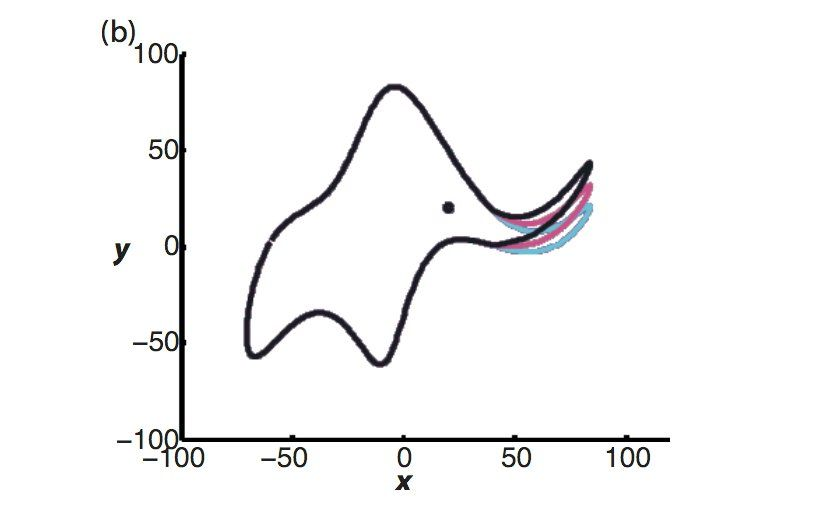
\includegraphics[width=0.6\textwidth]{IMG/Elephant.jpg}
\end{figure}
\centering
\textcolor{blue}{\underline{\href{https://fermatslibrary.com/s/drawing-an-elephant-with-four-complex-parameters}{Drawing an elephant with four complex parameters}}}
\end{frame}
%---------------------------------------------
\end{document}